\documentclass[12pt]{article}
\usepackage[margin=1in]{geometry}
\usepackage{graphicx}
\usepackage{booktabs}
\usepackage{amsmath}
\usepackage{amssymb}
\usepackage{bm}
\usepackage{float}
\usepackage{caption}
\usepackage{setspace}
\usepackage{tikz}
\usepackage{xcolor}
\usepackage{algorithm}
\usepackage{algpseudocode}
\usepackage[most]{tcolorbox}
\usepackage{hyperref}
\usetikzlibrary{arrows.meta, calc, positioning, backgrounds}
\captionsetup{font=small, labelfont=bf, skip=6pt}
\captionsetup[algorithm]{labelformat=empty, name={}}
\onehalfspacing
\hypersetup{hidelinks}
\setcounter{tocdepth}{2}
\graphicspath{%
  {../eda/figures/}%
  {../feature_eng/figures/}%
  {../eval_freeze/figures/}%
  {../models/figures/}%
  {figures/rnn_lstm/}%
  {figures/insea/}%
  {figures/}%
}

\definecolor{MITgreen}{HTML}{C0E0B0}
\definecolor{MITblue}{HTML}{B0D0E0}
\definecolor{MITpurple}{HTML}{D0B0F0}
\definecolor{inseadg}{HTML}{018754}
\definecolor{insealg}{HTML}{79b695}
\definecolor{inseawg}{HTML}{c4dcce}
\tikzset{background rectangle/.style={thin, draw=insealg, fill=inseawg, rounded corners=1ex}}

\newtcolorbox{explain}{%
  colback=black!3,
  colframe=black!25,
  boxrule=0.5pt,
  arc=1pt,
  left=8pt,
  right=8pt,
  top=5pt,
  bottom=5pt,
  before skip=6pt,
  after skip=12pt,
  fontupper=\normalsize
}

\title{Bitcoin Volatility Prediction Using Gated Recurrent Neural Networks}
\author{Abderrahmane Naitelhaj}
\date{30 September 2026}

\begin{document}

\begin{titlepage}
\thispagestyle{empty}
\newgeometry{left=0pt, right=0pt, top=20pt, bottom=0pt}
\begin{tikzpicture}[remember picture, overlay, yshift=5cm, every path/.style={inseadg}]
  \draw ([xshift=6.5cm]current page.north west) .. controls ([xshift=6.25cm,yshift=-4cm]current page.north west) and ([xshift=1cm,yshift=-5cm]current page.north west) .. ([yshift=-8.5cm]current page.north west);
  \draw ([xshift=7cm]current page.north west) .. controls ([xshift=6.75cm,yshift=-4cm]current page.north west) and ([xshift=1cm,yshift=-5cm]current page.north west) .. ([yshift=-9cm]current page.north west);
  \draw ([xshift=7.5cm]current page.north west) .. controls ([xshift=7.25cm,yshift=-4cm]current page.north west) and ([xshift=1cm,yshift=-5cm]current page.north west) .. ([yshift=-9.5cm]current page.north west);
  \draw ([xshift=8cm]current page.north west) .. controls ([xshift=7.75cm,yshift=-4cm]current page.north west) and ([xshift=1cm,yshift=-5cm]current page.north west) .. ([yshift=-10cm]current page.north west);
  \draw ([xshift=8.5cm]current page.north west) .. controls ([xshift=8.25cm,yshift=-4cm]current page.north west) and ([xshift=1cm,yshift=-5cm]current page.north west) .. ([yshift=-10.5cm]current page.north west);
  \draw ([xshift=9cm]current page.north west) .. controls ([xshift=8.75cm,yshift=-4cm]current page.north west) and ([xshift=1cm,yshift=-5cm]current page.north west) .. ([yshift=-11cm]current page.north west);
  \draw ([xshift=9.5cm]current page.north west) .. controls ([xshift=9.25cm,yshift=-4cm]current page.north west) and ([xshift=1cm,yshift=-5cm]current page.north west) .. ([yshift=-11.5cm]current page.north west);
  \draw ([xshift=10cm]current page.north west) .. controls ([xshift=9.75cm,yshift=-4cm]current page.north west) and ([xshift=1cm,yshift=-5cm]current page.north west) .. ([yshift=-12cm]current page.north west);
\end{tikzpicture}
\begin{center}
  
\includegraphics[width=100pt, trim={0 0 0 1.5cm}, clip]{hcp.png}
  \begin{minipage}{.6\textwidth}
    \vspace*{-60pt}
    \centering\scshape Royaume du Maroc\\
    Haut Commissariat au Plan\\
    Institut National de Statistique \\et d'\'Economie Appliqu\'ee\\[1.5ex]
    {\Huge \color{insealg} INSEA}
  \end{minipage}
  \vspace*{2\baselineskip}
  
\includegraphics[width=60pt, angle=1, origin=c]{logo.png}

  \vfill

  \rule{0.85\textwidth}{0.4pt}\\[0.9em]
  {\bfseries\LARGE Bitcoin Volatility Prediction\\[0.35em]
  Using Gated Recurrent Neural Networks}\\[0.9em]
  \rule{0.85\textwidth}{0.4pt}

  \vfill
  \begin{minipage}{.6\textwidth}\centering
    \begin{tabular}{l@{ \textbf{:} }l}
      \textbf{Author} & Abderrahmane Naitelhaj \\
      \textbf{Date} & 30 September 2026 \\
    \end{tabular}
  \end{minipage}
  \vfill
\end{center}
\begin{tikzpicture}[remember picture, overlay, shift={(current page.south west)}, every path/.style={inseadg}]
  \path [fill=inseadg] ([xshift=-6cm]current page.south east) .. controls ([xshift=-5.75cm,yshift=4cm]current page.south east) and ([xshift=-1cm,yshift=5cm]current page.south east) .. ([yshift=8cm]current page.south east) -- (current page.south east) -- cycle;
  \draw ([xshift=-6.5cm]current page.south east) .. controls ([xshift=-6.25cm,yshift=4cm]current page.south east) and ([xshift=-1cm,yshift=5cm]current page.south east) .. ([yshift=8.5cm]current page.south east);
  \draw ([xshift=-7cm]current page.south east) .. controls ([xshift=-6.75cm,yshift=4cm]current page.south east) and ([xshift=-1cm,yshift=5cm]current page.south east) .. ([yshift=9cm]current page.south east);
  \draw ([xshift=-7.5cm]current page.south east) .. controls ([xshift=-7.25cm,yshift=4cm]current page.south east) and ([xshift=-1cm,yshift=5cm]current page.south east) .. ([yshift=9.5cm]current page.south east);
  \draw ([xshift=-8cm]current page.south east) .. controls ([xshift=-7.75cm,yshift=4cm]current page.south east) and ([xshift=-1cm,yshift=5cm]current page.south east) .. ([yshift=10cm]current page.south east);
  \draw ([xshift=-8.5cm]current page.south east) .. controls ([xshift=-8.25cm,yshift=4cm]current page.south east) and ([xshift=-1cm,yshift=5cm]current page.south east) .. ([yshift=10.5cm]current page.south east);
  \draw ([xshift=-9cm]current page.south east) .. controls ([xshift=-8.75cm,yshift=4cm]current page.south east) and ([xshift=-1cm,yshift=5cm]current page.south east) .. ([yshift=11cm]current page.south east);
  \draw ([xshift=-9.5cm]current page.south east) .. controls ([xshift=-9.25cm,yshift=4cm]current page.south east) and ([xshift=-1cm,yshift=5cm]current page.south east) .. ([yshift=11.5cm]current page.south east);
  \draw ([xshift=-10cm]current page.south east) .. controls ([xshift=-9.75cm,yshift=4cm]current page.south east) and ([xshift=-1cm,yshift=5cm]current page.south east) .. ([yshift=12cm]current page.south east);
\end{tikzpicture}
\restoregeometry
\end{titlepage}

\thispagestyle{empty}
\vspace*{\stretch{1}}
\begin{center}
{\Large\bfseries Abstract}
\end{center}
\vspace{1.25em}
\begin{quote}
\noindent
Volatility forecasts support risk limits, sizing, and any decision that depends on how large price moves are likely to be.
This report asks whether deep learning can improve one-day-ahead Bitcoin realized-volatility forecasts relative to classical time-series models.
Daily realized volatility is built from hourly Binance BTC/USDT log returns; the modeling target is next-day \(\log\mathrm{RV}\).
Under one frozen chronological train/validation/test protocol, a lag-1 Naive rule, ARIMA, and HAR are compared with a standalone LSTM.
GARCH on daily returns is kept only as a conditional-volatility reference and is not part of the final realized-volatility ladder.
Accuracy is scored by RMSE and MAE on \(\log\mathrm{RV}\) and by MAPE and QLIKE on RV.
On the test window the standalone LSTM is close to HAR and significantly better only on MAPE, which motivates a hybrid that freezes the HAR fit and trains an LSTM on the residual.
That hybrid improves on both HAR and the standalone LSTM across the reported metrics.
A short primer on recurrent networks and LSTMs precedes the forecasting experiments.
\end{quote}
\vspace*{\stretch{2}}
\clearpage

\tableofcontents
\clearpage

\section{Introduction}
Volatility is the scale of price uncertainty. A usable forecast of how large moves are likely to be matters for risk limits, position sizing, option pricing, and any rule that widens or tightens when markets are calm versus stressed.
Bitcoin is a natural stress case: it trades continuously, swings hard, and has a long enough high-frequency record that daily realized volatility can be measured from intraday returns rather than inferred only from a daily close.

The practical goal of this work is to forecast that next-day realized volatility.
Classical time-series tools already do this job with a small number of parameters and a clear structure---persistence, multi-horizon averages, and return-based conditional variance.
The open question is whether deep learning, and in particular recurrent architectures built for sequences, can improve on those classical forecasts for the same target and the same out-of-sample protocol.

\section{Data}
Hourly BTC/USDT bars come from Binance spot, 17 August 2017 through 27 September 2026 (79{,}754 rows). Exact duplicate timestamps were dropped. Missing hours were not filled. Twenty-eight breaks longer than one hour are flagged and stored separately.

An hourly log return is kept only when the previous bar is exactly one hour earlier. A UTC day is complete when it has 24 valid hourly log returns: 3{,}298 such days, from 18 August 2017 to 26 September 2026. Incomplete days stay in the daily file and are flagged; they do not enter the model panel.

\[
r_{t,i}=\ln\Bigl(\frac{P_{t,i}}{P_{t,i-1}}\Bigr),
\qquad
\mathrm{RV}_t=\sqrt{\sum_{i\in t} r_{t,i}^2},
\qquad
R_t=\sum_{i\in t} r_{t,i}.
\]

\section{Exploratory data analysis}
Binance \texttt{BTC/USDT}. Complete UTC days only (24 valid hourly log returns; no gap fill).
Full sample: 3{,}298 days from 18 August 2017 to 26 September 2026.
Time-series plots use 1 January 2025 through the last complete day.
Histograms, moments, ACF/PACF, and ADF tests use the full sample.

\subsection{Closing price and volume}
\begin{figure}[H]
\centering
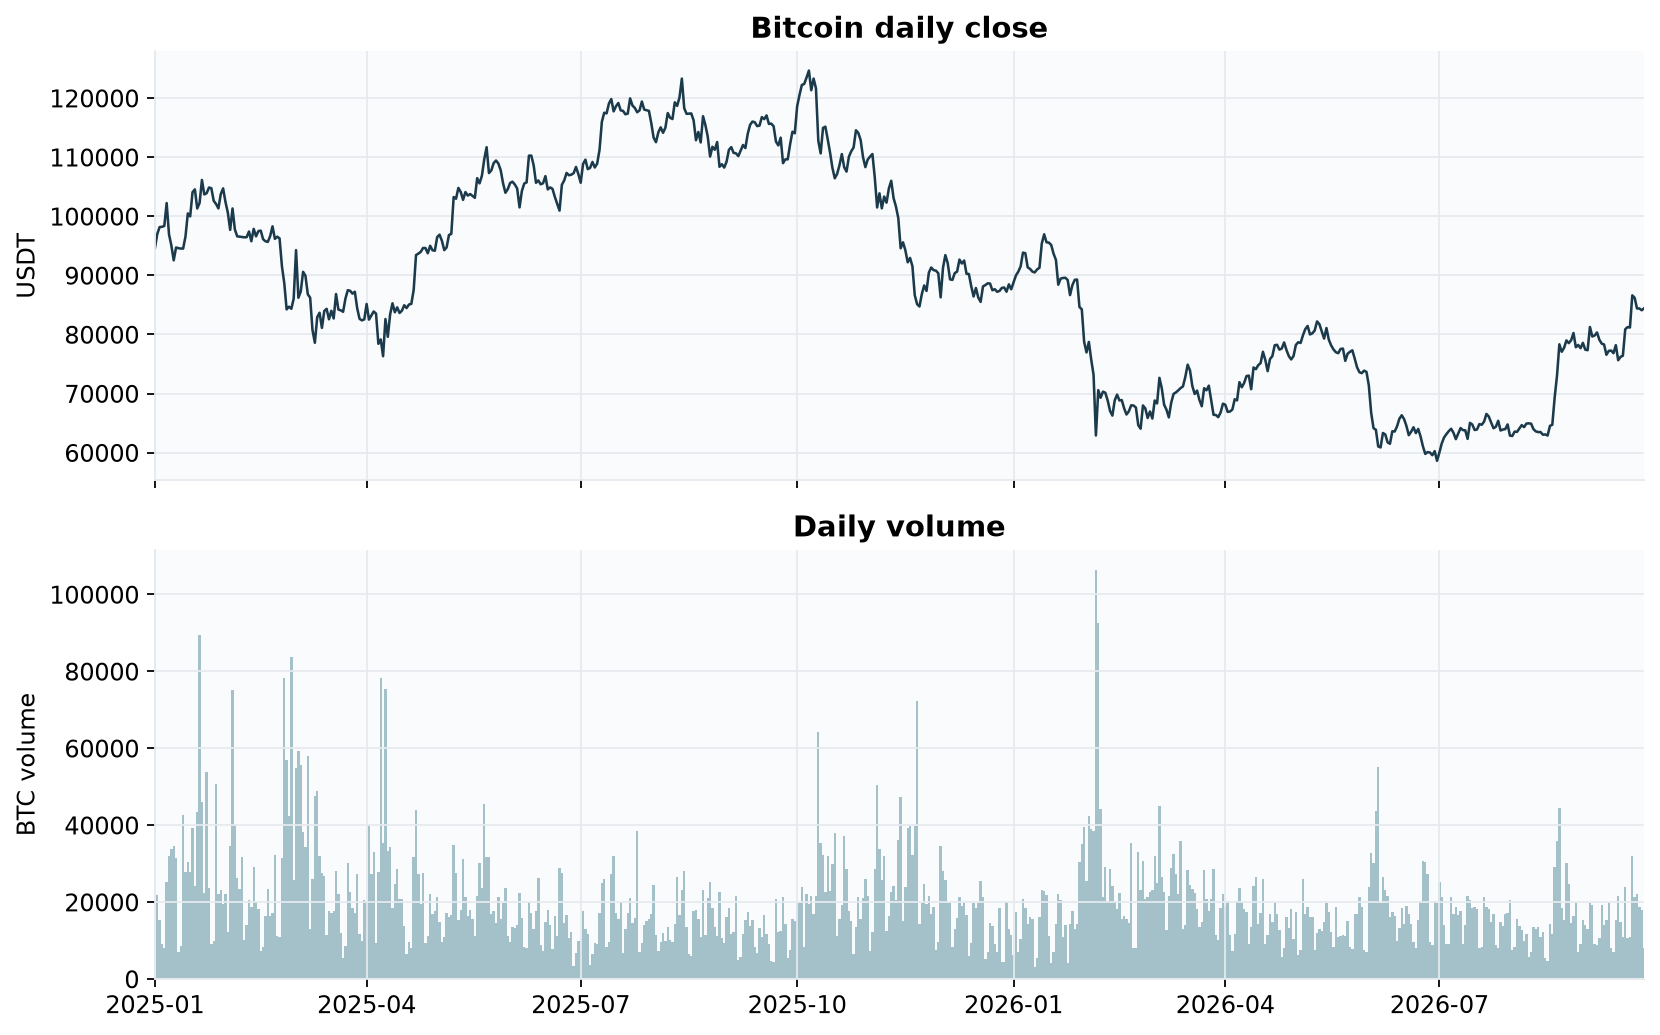
\includegraphics[width=\textwidth]{price_volume.png}
\caption{Daily closing price and trading volume.}
\end{figure}
\begin{explain}
Price and volume set the market context for the volatility series. Volume spikes often line up with sharp price moves, which is consistent with activity concentrating in turbulent episodes rather than arriving uniformly.
\end{explain}

\subsection{Volume \(z\)-score}
\[
Z^{(30)}_t=\frac{V_t-\mu^{(30)}_t}{\sigma^{(30)}_t}.
\]
\begin{figure}[H]
\centering
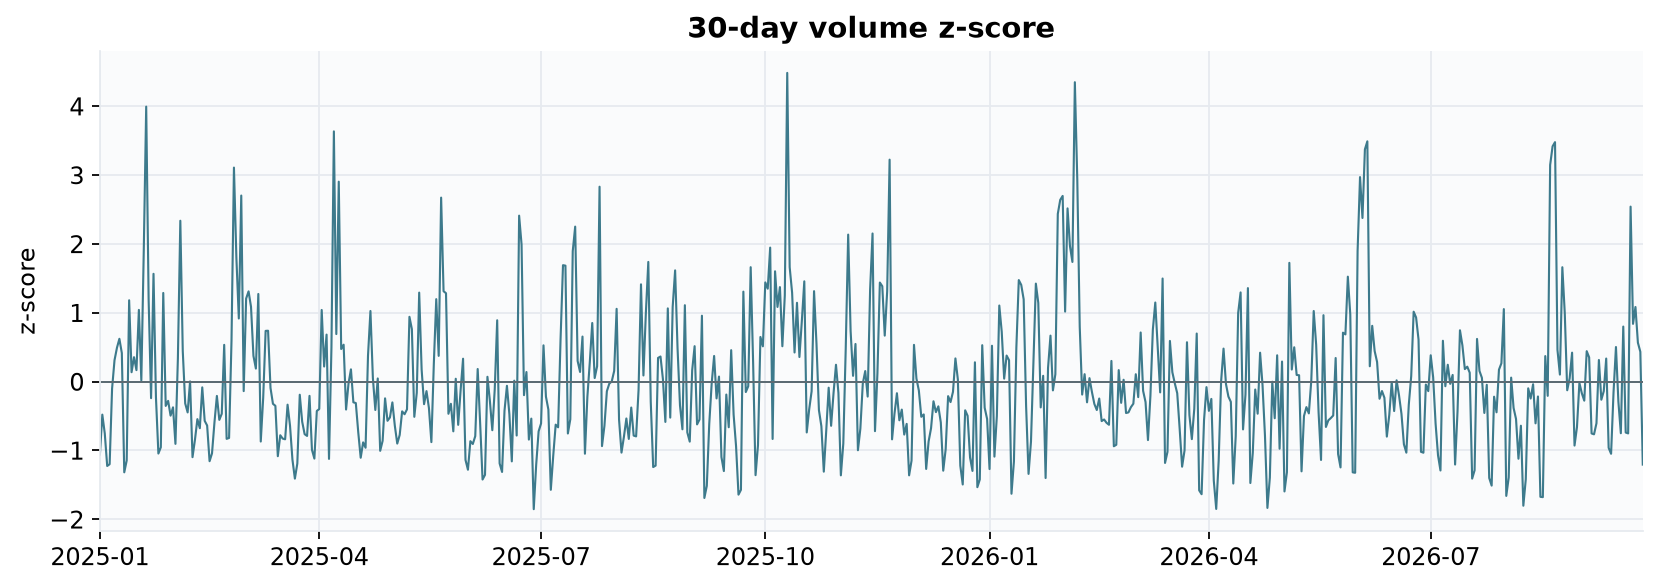
\includegraphics[width=\textwidth]{volume_z.png}
\caption{30-day volume \(z\)-score.}
\end{figure}
\begin{explain}
Large \(|z|\) flags days that are unusually busy or quiet relative to the recent month. Such activity shocks often accompany volatility bursts and are a natural candidate covariate alongside lagged \(\mathrm{RV}\).
\end{explain}

\subsection{Logarithmic returns}
\[
r_{t,i}=\ln\Bigl(\frac{P_{t,i}}{P_{t,i-1}}\Bigr),
\qquad
R_t=\sum_{i\in t} r_{t,i}.
\]
\begin{figure}[H]
\centering
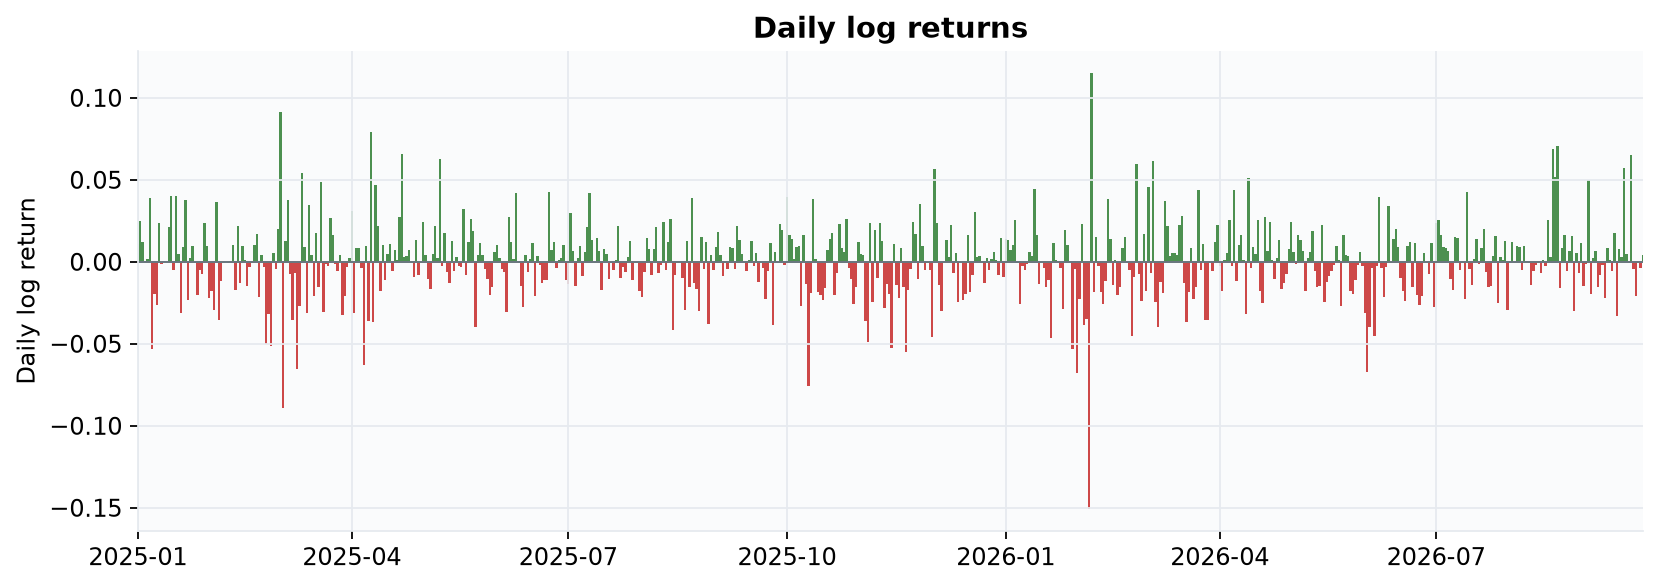
\includegraphics[width=\textwidth]{daily_log_returns.png}
\caption{Daily log returns.}
\end{figure}
\begin{explain}
Daily returns oscillate around zero with frequent large moves of both signs. The path is noisy and only weakly predictable from its own lags; the interesting structure lives in the size of those moves---volatility---rather than in the sign of \(R_t\).
\end{explain}

\subsection{Distribution of logarithmic returns}
\begin{figure}[H]
\centering
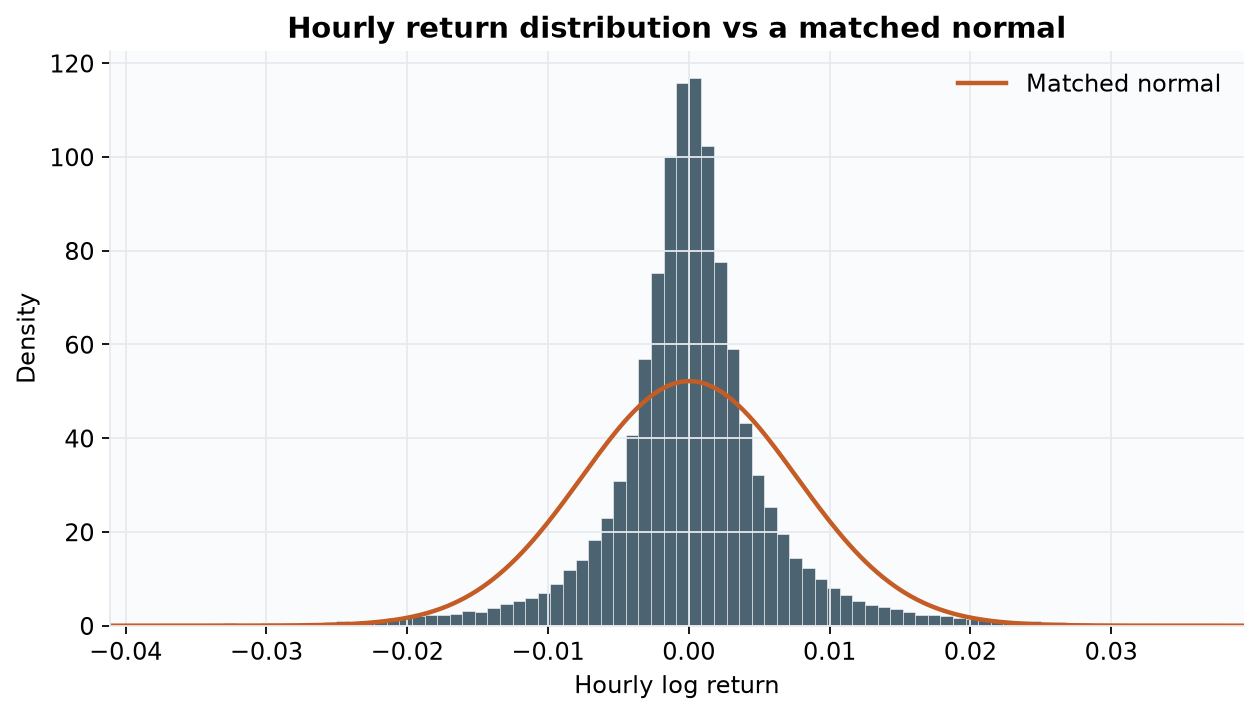
\includegraphics[width=0.92\textwidth]{return_hist.png}
\caption{Distribution of hourly log returns versus a matched normal.}
\end{figure}
\begin{explain}
Hourly log returns---the building blocks of \(\mathrm{RV}_t\)---are heavy-tailed relative to a matched normal (skewness about \(-0.47\), excess kurtosis about \(37\)). Large gains and losses are far more common than Gaussian theory allows. The time-series and ACF panels use daily returns for readability; the histogram keeps the hourly grain because aggregation is not needed for a density plot.
\end{explain}

\subsection{Autocorrelation of logarithmic returns}
ACF and PACF are shown with lag~0 equal to 1 and vertical axis on \([-1,1]\). The shaded band is \(\pm 1.96/\sqrt{n}\approx\pm 0.034\).
\begin{figure}[H]
\centering
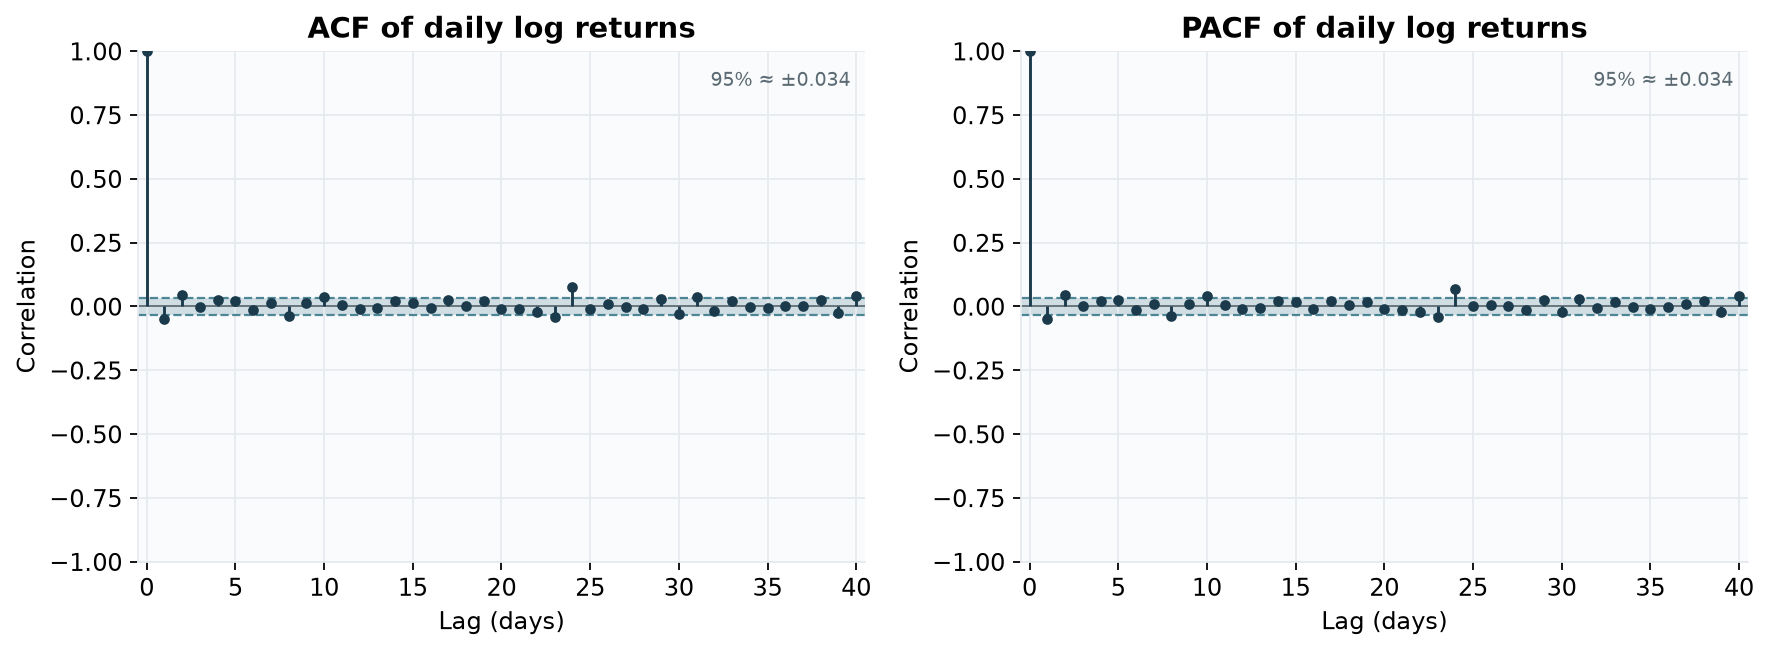
\includegraphics[width=\textwidth]{acf_pacf_returns.png}
\caption{ACF and PACF of daily log returns.}
\end{figure}
\begin{explain}
After lag~0, autocorrelations are small. An ADF test rejects a unit root (statistic \(-11.07\), \(p\approx 4.6\times 10^{-20}\)): returns look stationary and only weakly dependent. The forecasting problem sits in volatility, not in predicting \(R_t\) from its own lags.
\end{explain}

\subsection{Rolling skewness and kurtosis}
\[
\mathrm{Skew}_t
=
\frac{\mathbb{E}[(r-\bar r)^3]}
{(\mathbb{E}[(r-\bar r)^2])^{3/2}},
\qquad
\mathrm{Kurt}_t
=
|\frac{\mathbb{E}[(r-\bar r)^4]}
{(\mathbb{E}[(r-\bar r)^2])^{2}}-3,
\]
computed over the last 30 days of hourly returns.
\begin{figure}[H]
\centering
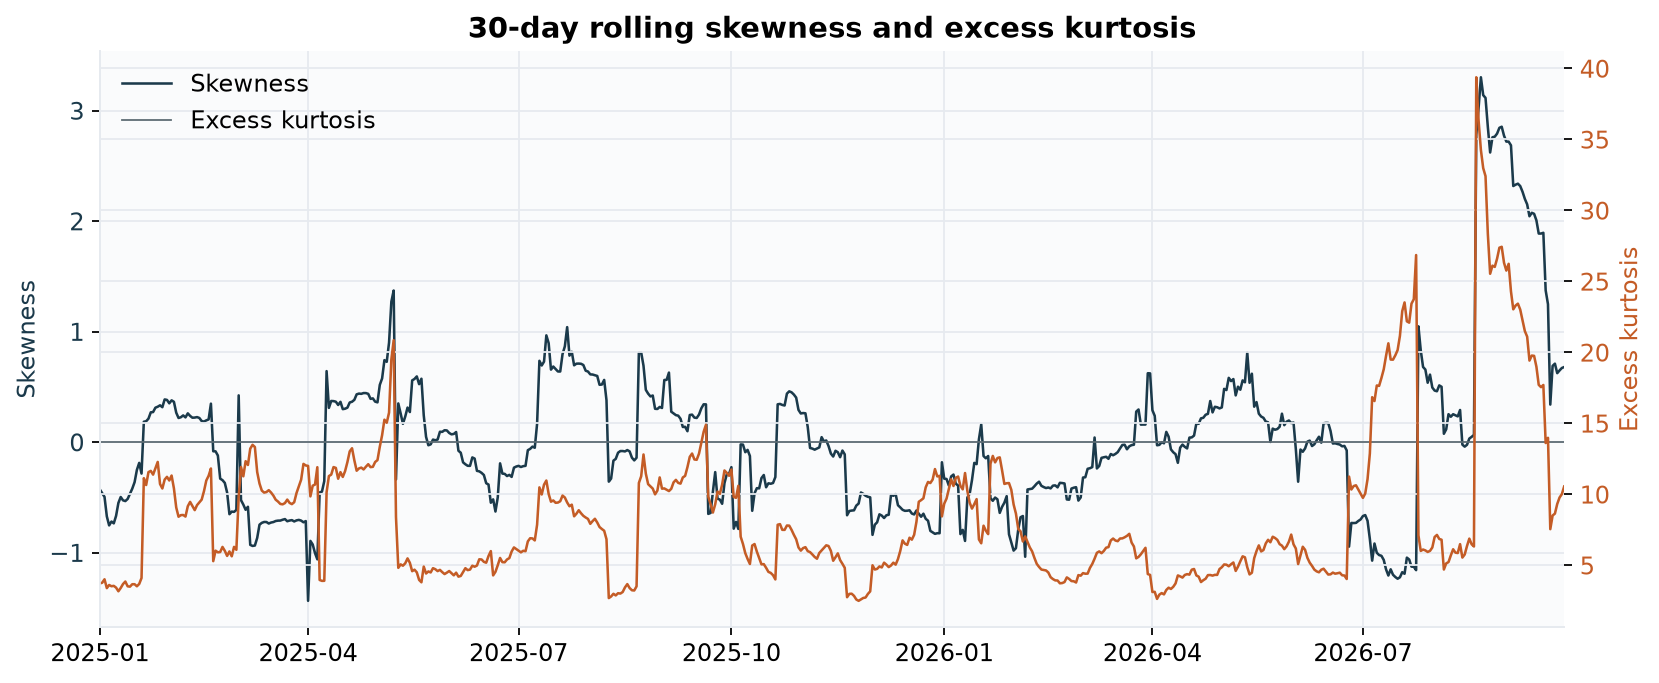
\includegraphics[width=\textwidth]{rolling_skew_kurt.png}
\caption{Rolling 30-day skewness and excess kurtosis of log returns (excess kurtosis $= $ kurtosis $-3$).}
\end{figure}
\begin{explain}
Spikes in excess kurtosis mark windows where extreme moves dominate; those episodes often coincide with high \(\mathrm{RV}\). Skewness shifts show whether recent extremes sit more on the downside or the upside. The two series use different vertical scales.
\end{explain}

\subsection{Realized volatility}
\[
\mathrm{RV}_t=\sqrt{\sum_{i\in t} r_{t,i}^2},
\qquad
\mathrm{RV}_t^{\mathrm{ann}}=\mathrm{RV}_t\sqrt{365}.
\]
\begin{figure}[H]
\centering
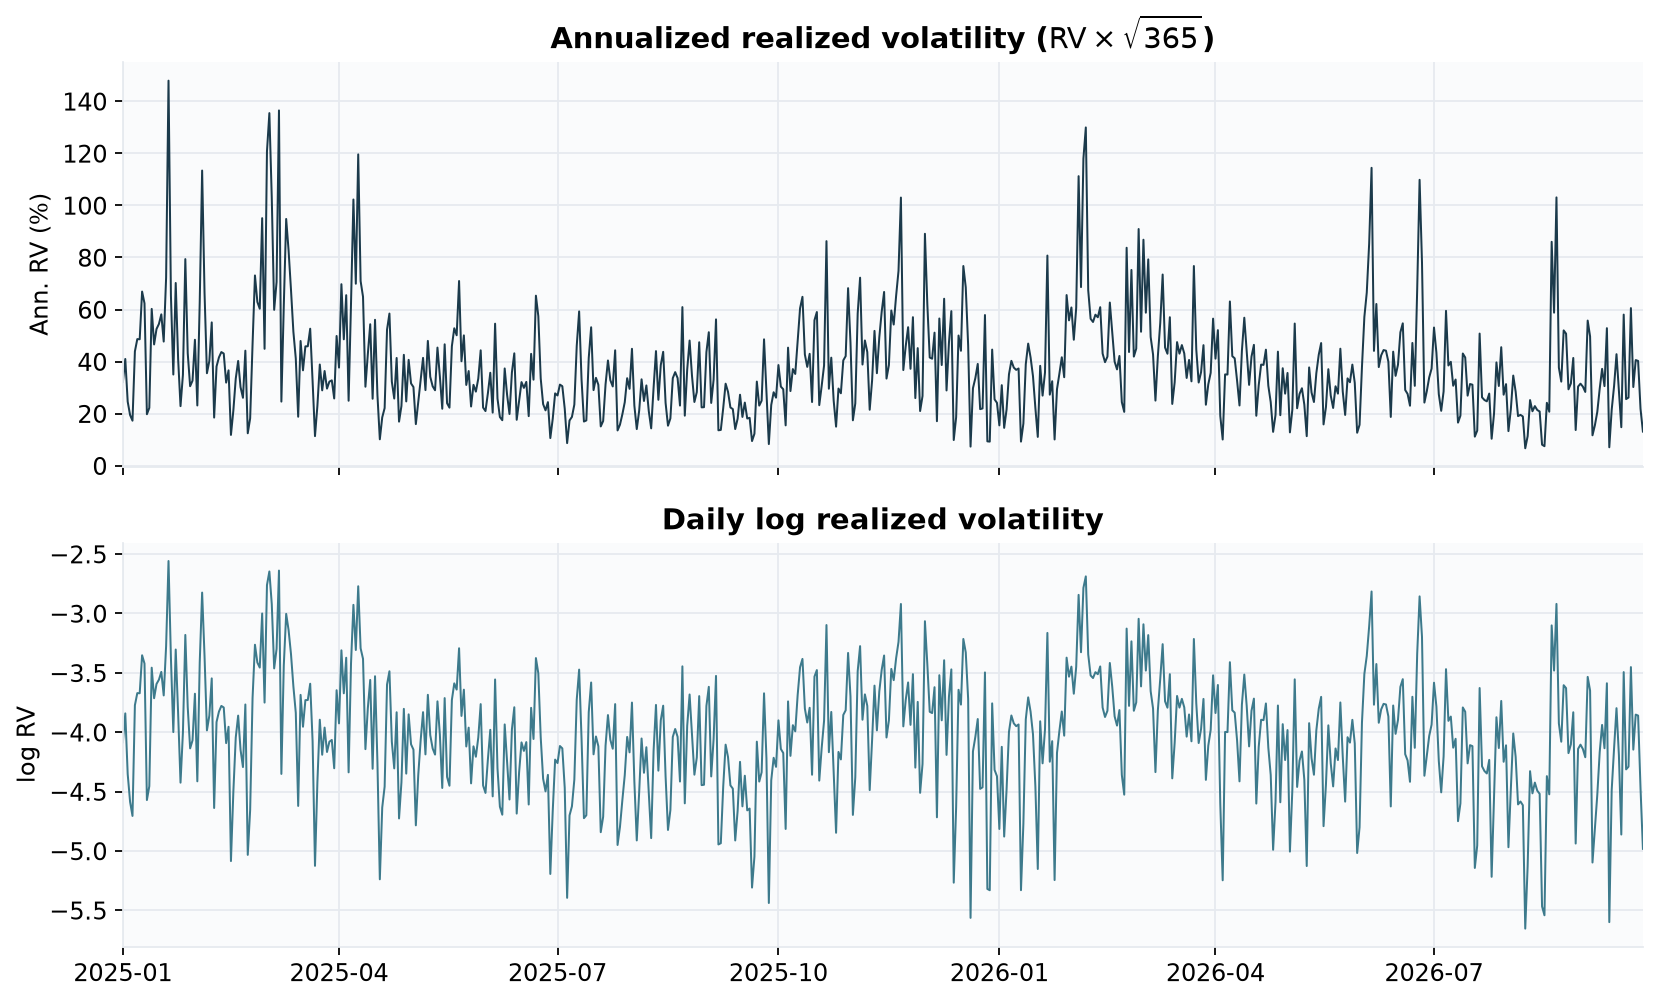
\includegraphics[width=\textwidth]{rv_timeseries.png}
\caption{Annualized daily realized volatility (\%) and \(\log\mathrm{RV}\).}
\end{figure}
\begin{explain}
High- and low-volatility stretches arrive in runs (clustering). The top panel is annualized so the level is readable as a yearly scale (\(100\times\mathrm{RV}\sqrt{365}\) percent); the bottom panel is \(\log\mathrm{RV}\), the smoother scale used for modeling. Full-sample mean annualized RV is about \(57\%\).
\end{explain}

\subsection{Distribution of RV and \(\log\mathrm{RV}\)}
\begin{figure}[H]
\centering
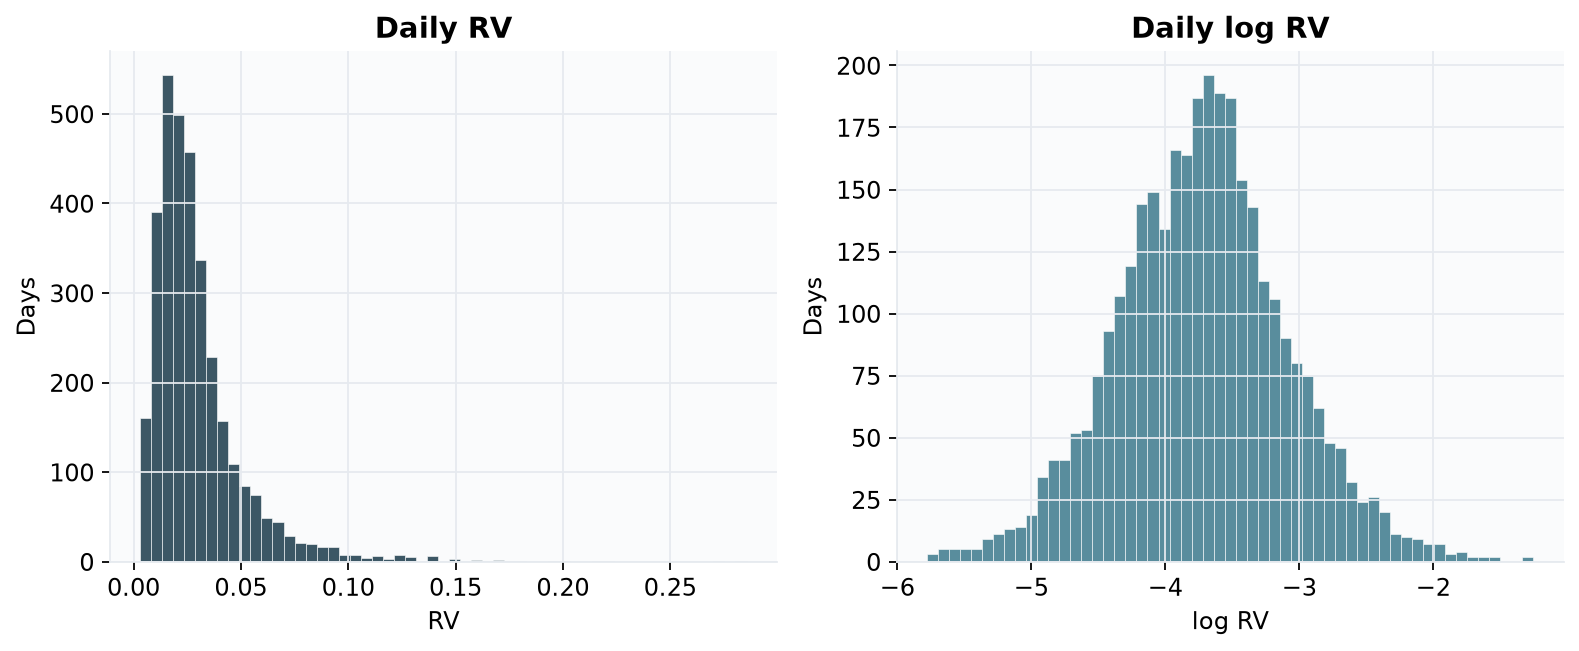
\includegraphics[width=\textwidth]{rv_hist.png}
\caption{Histograms of daily RV and of \(\log\mathrm{RV}\).}
\end{figure}
\begin{explain}
Raw RV is strongly right-skewed (skewness \(3.21\)). \(\log\mathrm{RV}\) is nearly symmetric (skewness \(0.08\), excess kurtosis \(0.36\)), which is a better scale for MSE-type losses and for linear or neural predictors of next-day volatility.
\end{explain}

\subsection{Autocorrelation of \(\log\mathrm{RV}\)}
\begin{figure}[H]
\centering
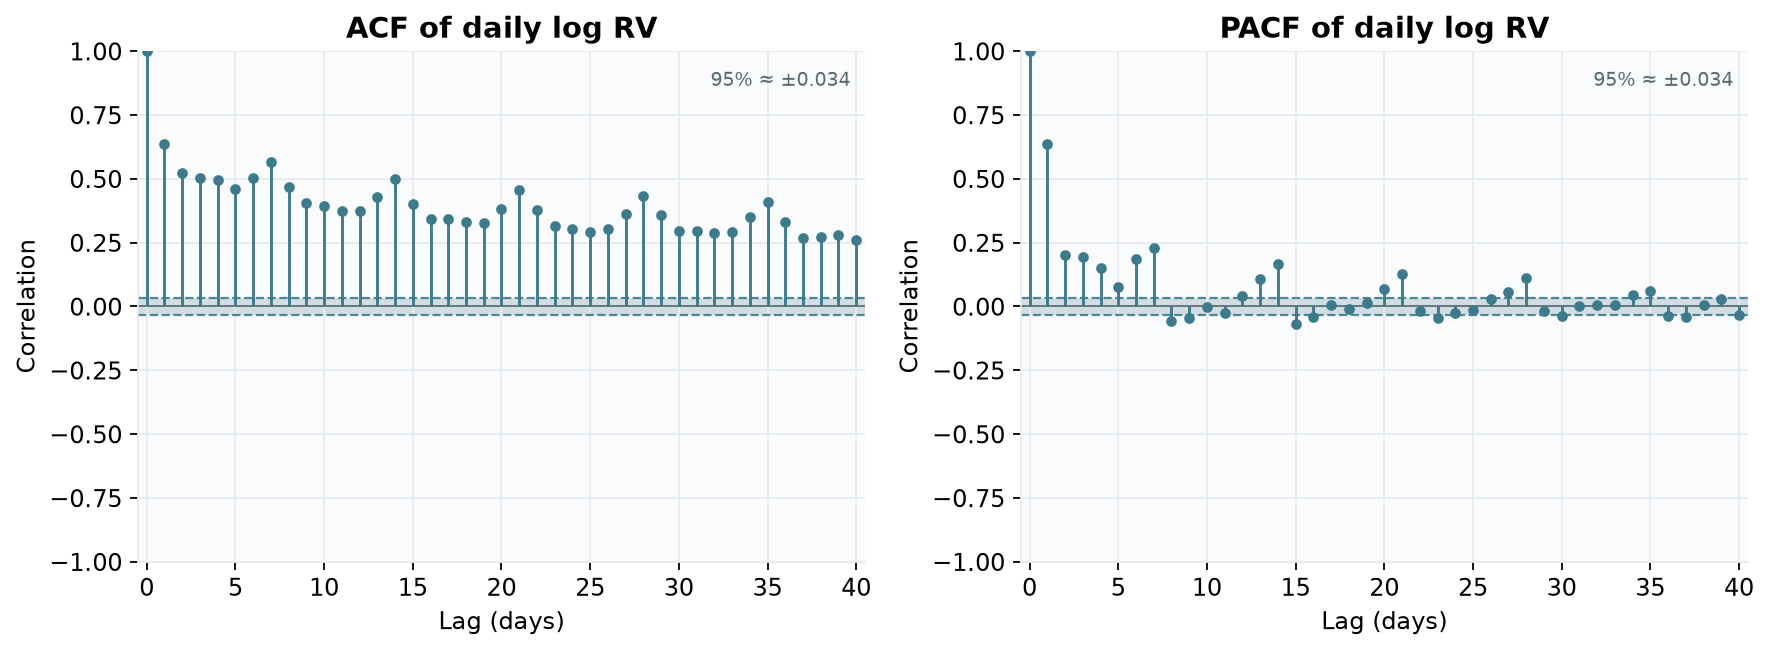
\includegraphics[width=\textwidth]{acf_pacf_log_rv.png}
\caption{ACF and PACF of daily \(\log\mathrm{RV}\).}
\end{figure}
\begin{explain}
The autocorrelation decays slowly (about \(0.63\) at lag~1, \(0.46\) at lag~5, \(0.38\) at lag~22). An ADF test still rejects a unit root (statistic \(-4.86\), \(p=4.2\times 10^{-5}\)): \(\log\mathrm{RV}\) is persistent but stationary. That persistence is the main forecasting signal.
\end{explain}

\subsection{Relative Strength Index}
\[
\mathrm{RSI}_t=100-\frac{100}{1+\mathrm{RS}_t},
\qquad
\mathrm{RS}_t=\frac{\text{average gain}}{\text{average loss}}
\quad(14\text{ days}).
\]
\begin{figure}[H]
\centering
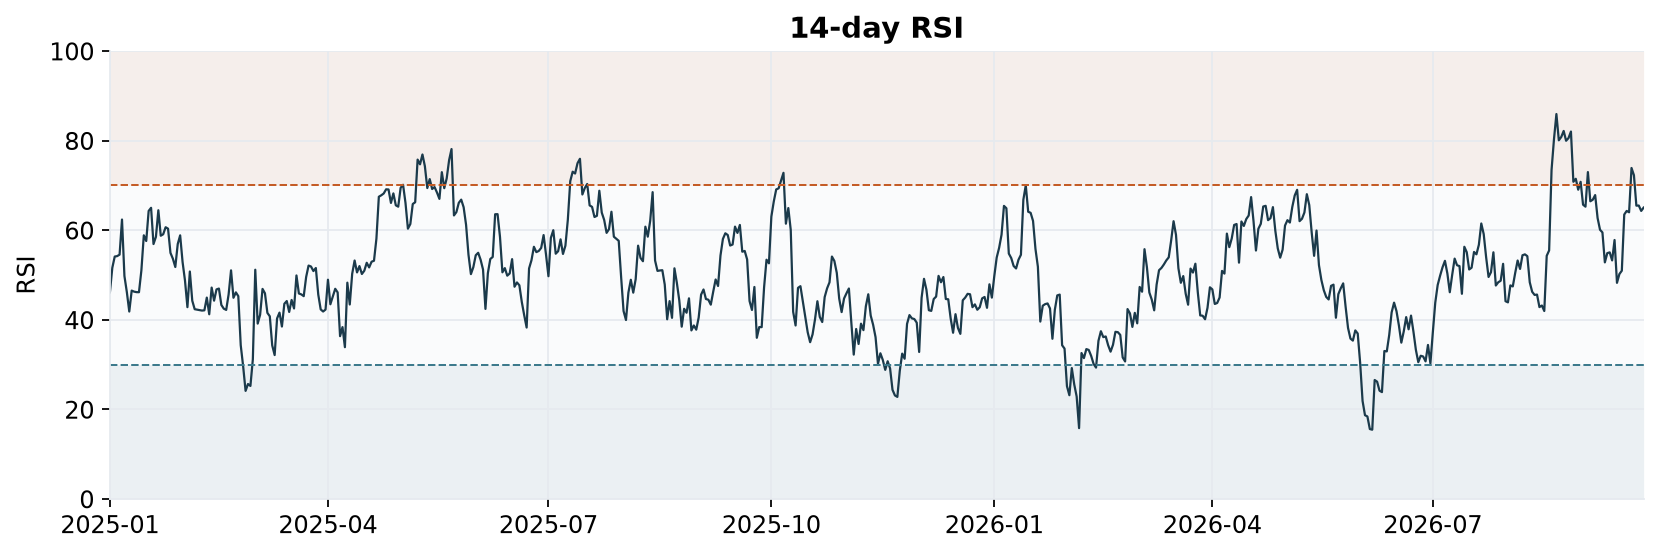
\includegraphics[width=\textwidth]{rsi.png}
\caption{14-day RSI.}
\end{figure}
\begin{explain}
RSI summarizes recent up versus down momentum. Readings above 70 and below 30 mark stretches that are strong relative to the last two weeks; here it is descriptive context, not a volatility forecast by itself.
\end{explain}

\subsection{Bollinger bands}
\[
\mathrm{Upper}_t=\mathrm{MA}^{(20)}_t+2\,\sigma^{(20)}_t,
\qquad
\mathrm{Lower}_t=\mathrm{MA}^{(20)}_t-2\,\sigma^{(20)}_t.
\]
\begin{figure}[H]
\centering
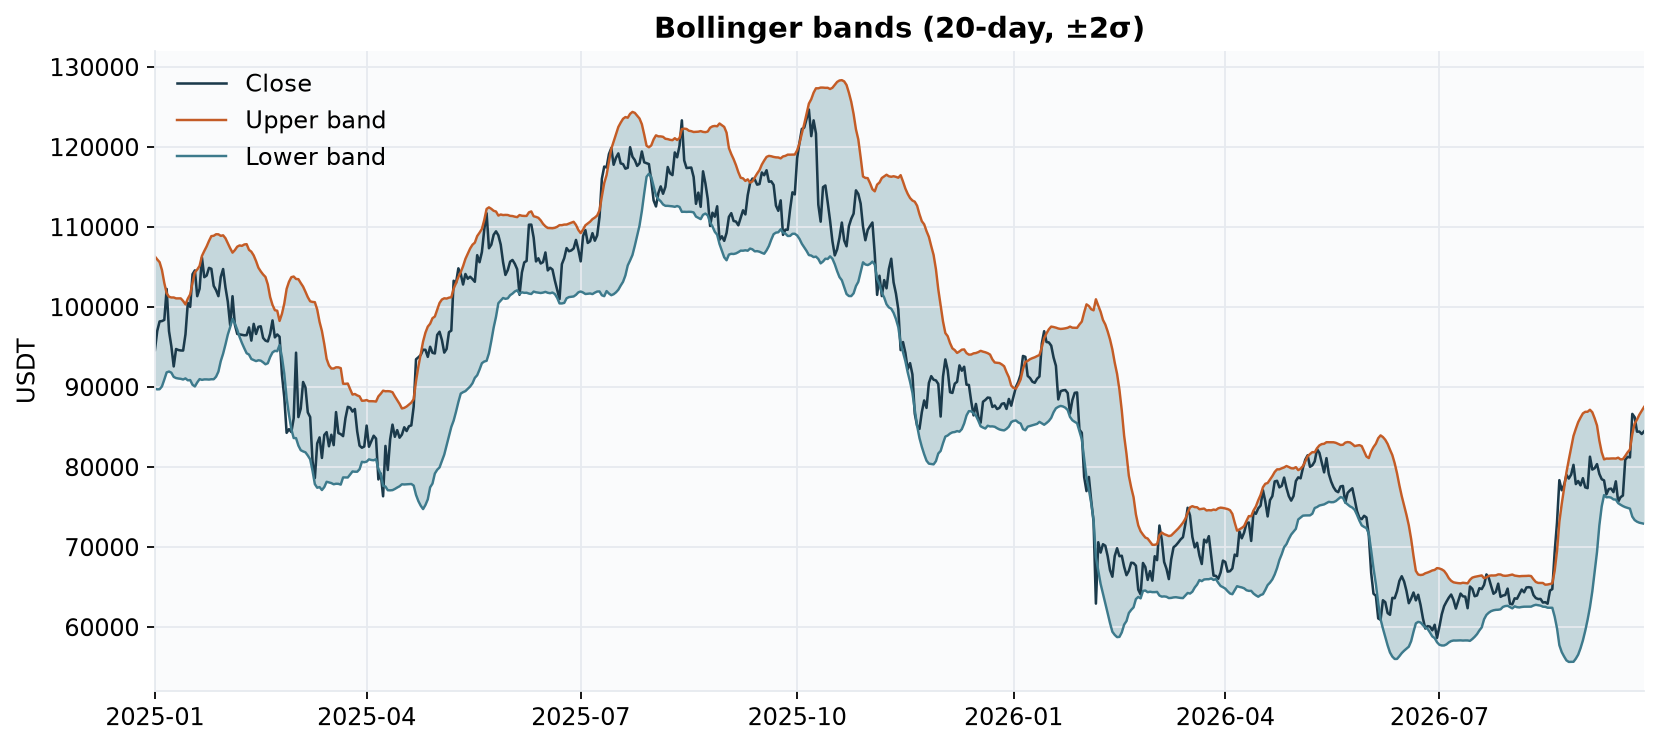
\includegraphics[width=\textwidth]{bollinger.png}
\caption{Closing price with 20-day Bollinger bands (\(\pm 2\sigma\)).}
\end{figure}
\begin{explain}
Band width is a rolling measure of local price dispersion: it widens in turbulent stretches and contracts in calm ones. Touches of the bands locate comparatively stretched prices within the recent 20-day window.
\end{explain}

\subsection{Synthesis}
Bitcoin returns are weakly autocorrelated and heavy-tailed. Daily realized volatility clusters and \(\log\mathrm{RV}\) is strongly persistent. The log transform removes the strong right skew of raw RV.

These facts support predicting one-day-ahead \(\log\mathrm{RV}\). Persistence points to lagged realized-volatility models; daily returns remain the natural input for a GARCH-style reference. A sequence model is evaluated later under the same chronological protocol (RMSE, MAE, MAPE, QLIKE).

\section{Target and features}
Only complete UTC days enter the panel (24 valid hourly log returns).
Everything at date \(t\) is known by the close of day \(t\).
RSI, Bollinger bands, rolling skewness/kurtosis, and price MAs stay in the exploratory section only.

\subsection{Target}
\[
y_t=\log\mathrm{RV}_{t+1},
\qquad
\mathrm{RV}_{t}=\sqrt{\sum_{i\in t} r_{t,i}^2}.
\]
\begin{figure}[H]
\centering
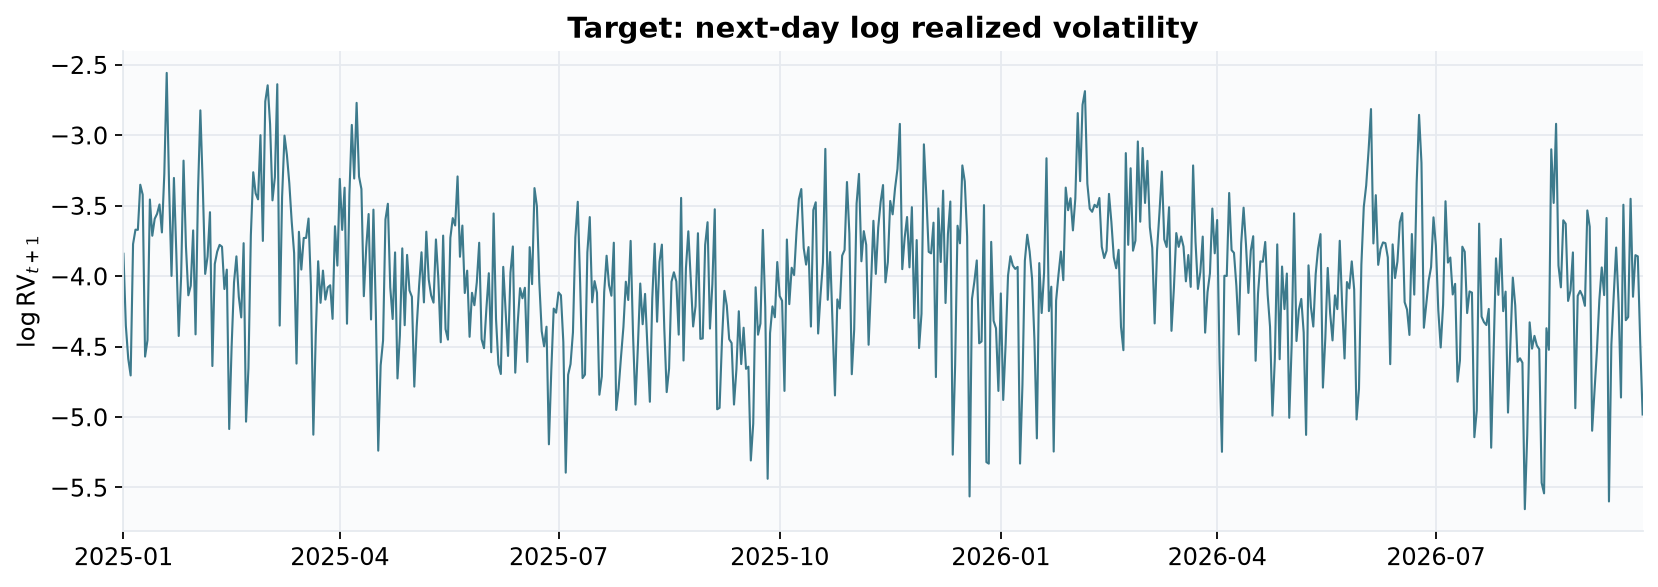
\includegraphics[width=\textwidth]{target_y.png}
\caption{Target series \(y_t=\log\mathrm{RV}_{t+1}\) (display window from 2025).}
\end{figure}
\begin{explain}
The project forecasts \(\log\mathrm{RV}_{t+1}\) (not price). Raw RV is right-skewed; \(\log\mathrm{RV}\) is nearly symmetric. The last day has no \(y_t\) because tomorrow's RV is unobserved.
\end{explain}

\subsection{Sample and leakage rules}
\begin{table}[H]
\centering
\begin{tabular}{lr}
\toprule
Complete UTC days & 3{,}298 \\
Model-ready rows & 3{,}268 \\
Dropped (warmup / no \(y\)) & 30 \\
HAR week window & 7 days \\
HAR month window & 22 days \\
Volume \(z\) window & 30 days \\
\bottomrule
\end{tabular}
\caption{Panel coverage after requiring a full lookback and a next-day target.}
\end{table}
\begin{explain}
Warmup drops come from the 30-day volume \(z\) and HAR windows; one final row is dropped because \(y_t\) needs day \(t+1\). No future information enters features at \(t\).
\end{explain}

\subsection{Who uses what}
Every model is scored against the same next-day realized volatility.
Naive, ARIMA, HAR, the LSTM, and the hybrid forecast \(y_t=\log\mathrm{RV}_{t+1}\) directly.
GARCH is fit on returns and emits conditional volatility \(\hat\sigma_{t+1}\), which is then scored against \(\mathrm{RV}_{t+1}\) (same outcome series, different forecast object).
What differs in the table is the \emph{input}, not the prediction task.
\begin{table}[H]
\centering
\begin{tabular}{ll}
\toprule
Model & Input \\
\midrule
Naive & \(\log\mathrm{RV}_t\) (lag-1 copy) \\
GARCH & daily return series \(R_t\) \\
ARIMA & \(\log\mathrm{RV}\) series \\
HAR & \(\log\mathrm{RV}^{(d)},\log\mathrm{RV}^{(w)},\log\mathrm{RV}^{(m)}\) \\
LSTM & length-\(L\) window of \(\log\mathrm{RV}\), its 7-day and 22-day means, \(R_t^2\), volume \(z\) \\
Hybrid & frozen HAR fit, then LSTM on the HAR residual \\
\bottomrule
\end{tabular}
\caption{Inputs by model. The evaluation target is next-day realized volatility for all of them.}
\end{table}
\begin{explain}
ARIMA and HAR are realized-vol-on-vol. The LSTM uses a short multivariate window. The hybrid keeps HAR's multi-horizon linear fit and trains the network only on what HAR misses. GARCH stays on the board only as a return-volatility reference; it is not part of the final RV ladder.
\end{explain}

\subsection{HAR-style log-RV features}
\[
\log\mathrm{RV}^{(d)}_t=\log\mathrm{RV}_t,
\quad
\log\mathrm{RV}^{(w)}_t=\frac1{7}\sum_{i=0}^{6}\log\mathrm{RV}_{t-i},
\quad
\log\mathrm{RV}^{(m)}_t=\frac1{22}\sum_{i=0}^{21}\log\mathrm{RV}_{t-i}.
\]
\begin{figure}[H]
\centering
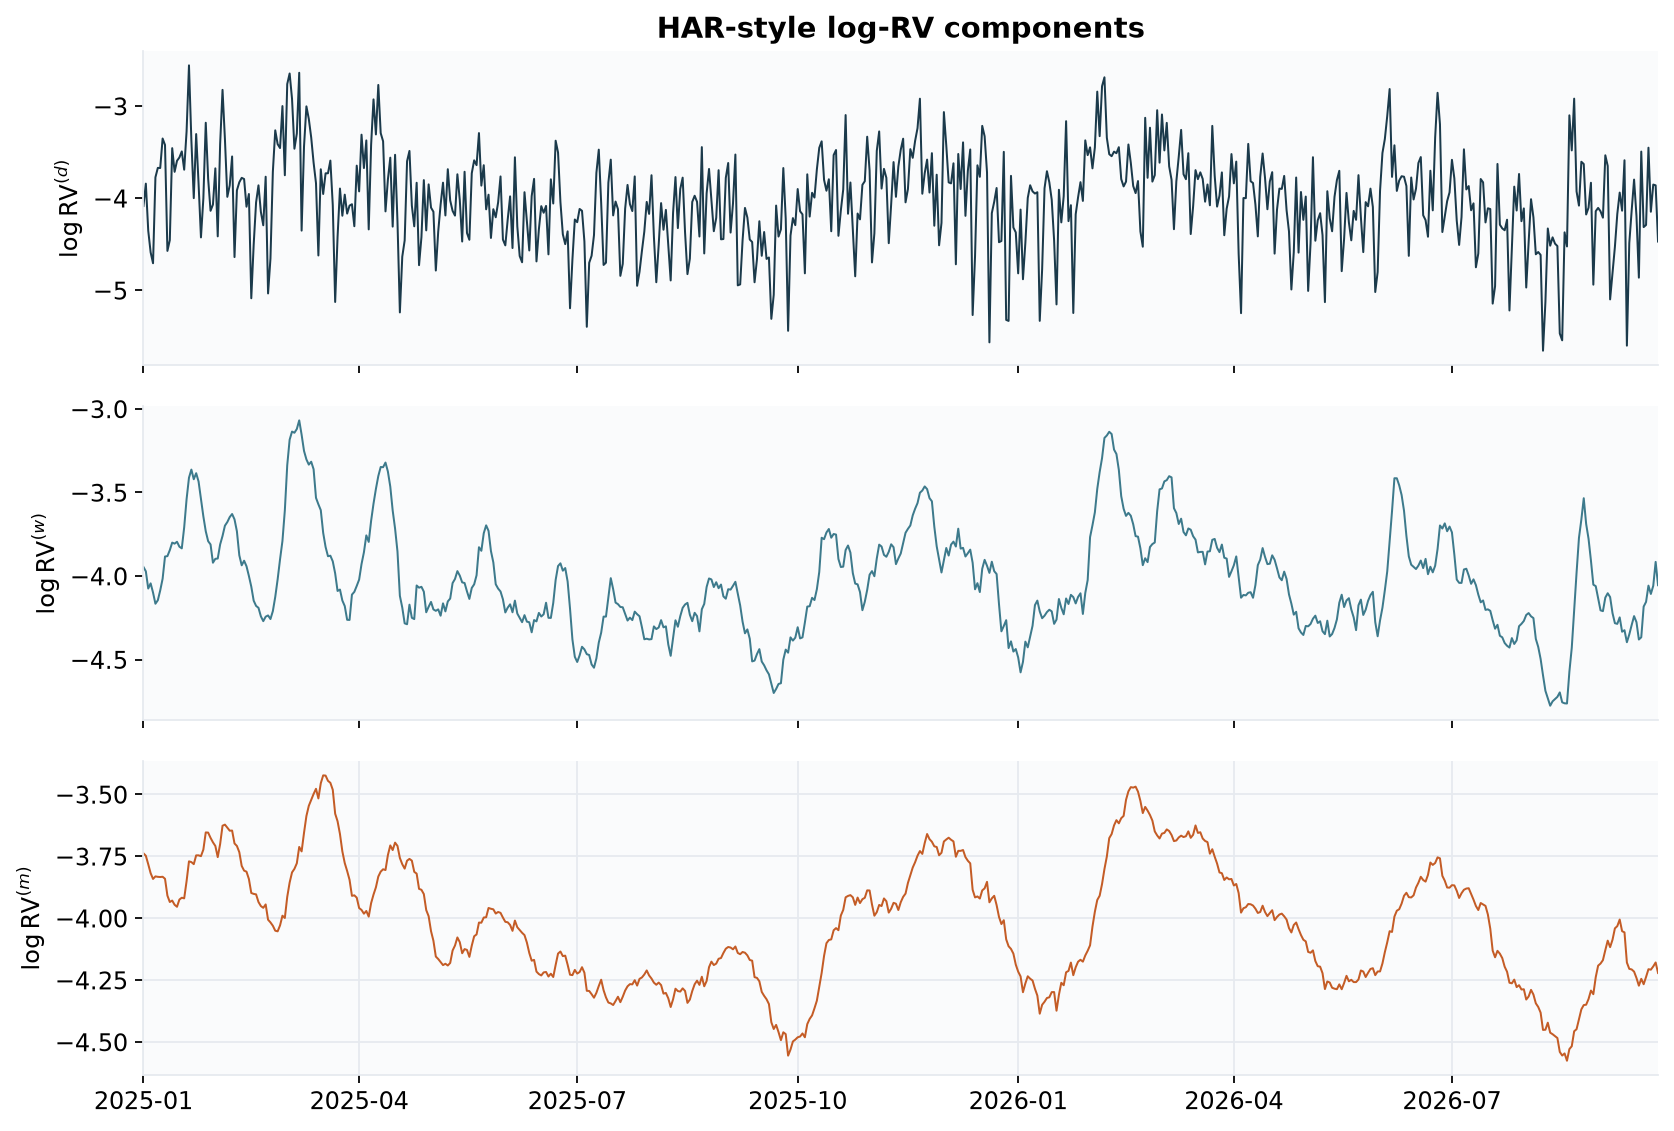
\includegraphics[width=\textwidth]{har_components.png}
\caption{Daily, weekly, and monthly log-RV components.}
\end{figure}
\begin{explain}
Crypto trades every calendar day, so the week average uses 7 days (not a 5-day equity week). The month term uses 22 days. These three terms are the HAR regressors. The same daily, weekly, and monthly series are channels in the LSTM window.
\end{explain}

\subsection{Returns}
\[
R_t=\sum_{i\in t} r_{t,i},
\qquad
R_t^2.
\]
\begin{figure}[H]
\centering
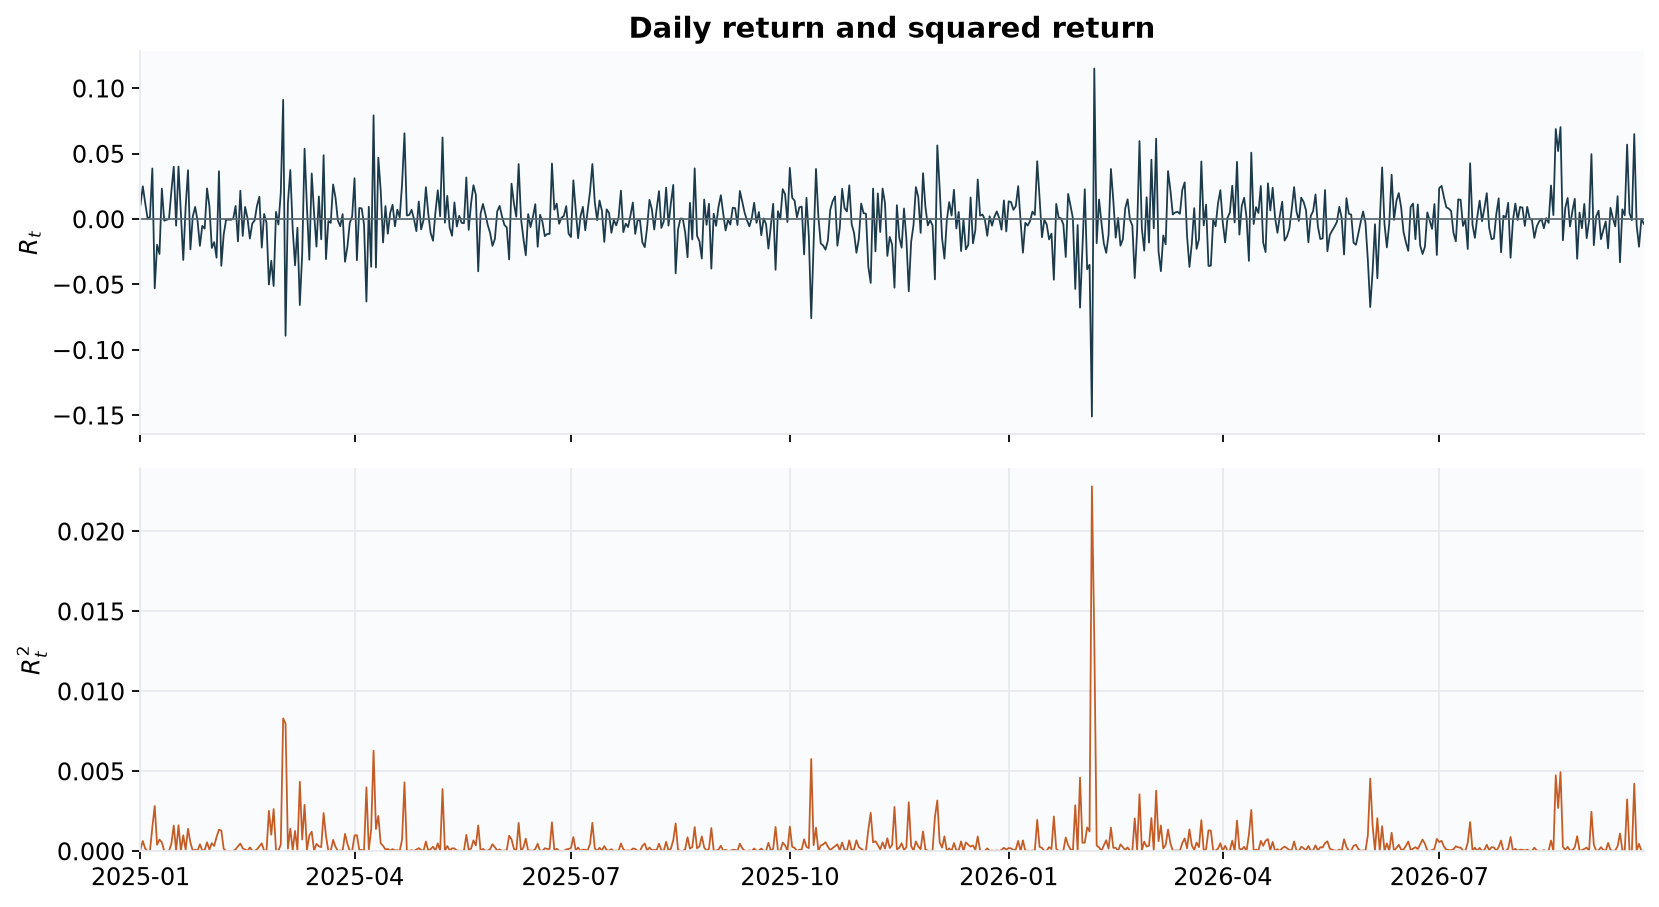
\includegraphics[width=\textwidth]{return_features.png}
\caption{Daily log return and squared return.}
\end{figure}
\begin{explain}
\(R_t\) is the input series for GARCH, not a HAR covariate. \(R_t^2\) is an LSTM channel (shock size). Signed \(R_t\) is a weak linear predictor of \(y_t\) and is not an LSTM channel.
\end{explain}

\subsection{Volume \(z\)-score}
\[
Z^{(30)}_t=\frac{V_t-\mu^{(30)}_t}{\sigma^{(30)}_t}.
\]
\begin{figure}[H]
\centering
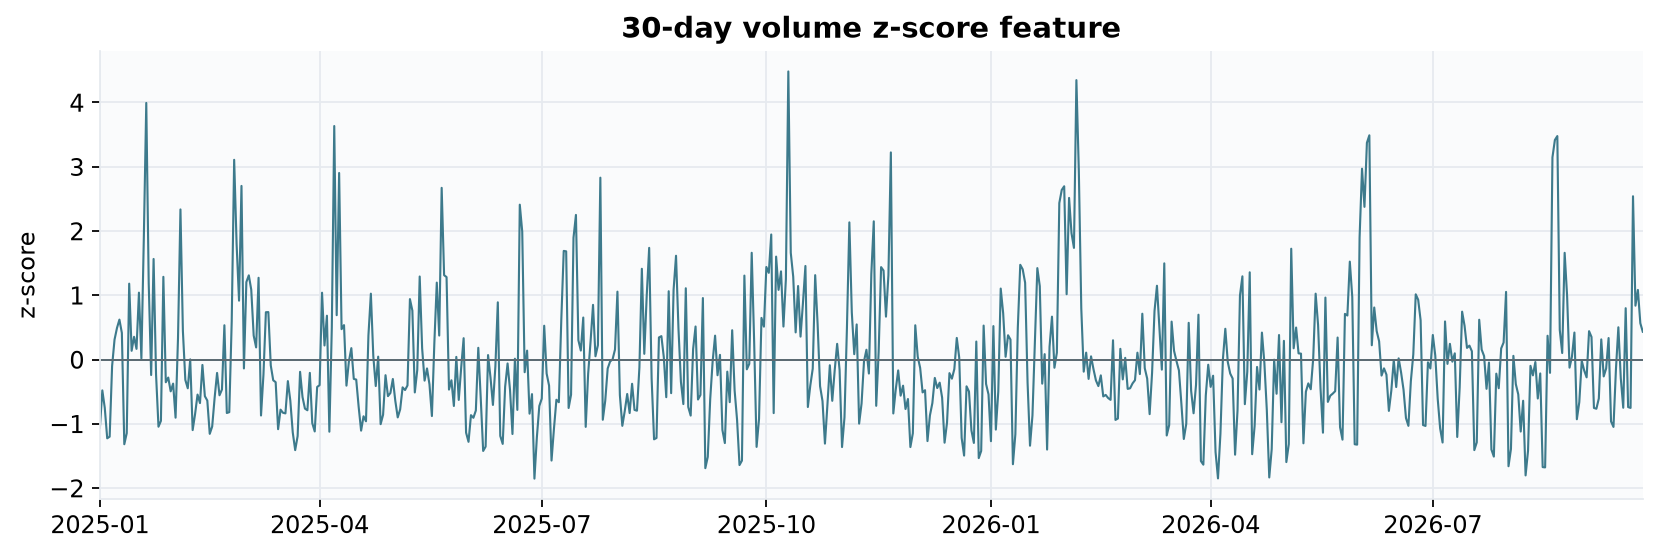
\includegraphics[width=\textwidth]{volume_z_feature.png}
\caption{30-day volume \(z\)-score.}
\end{figure}
\begin{explain}
Activity shocks often accompany volatility bursts. The series is an LSTM channel. It is not used by HAR, ARIMA, or GARCH.
\end{explain}

\subsection{Feature--target association}
\begin{figure}[H]
\centering
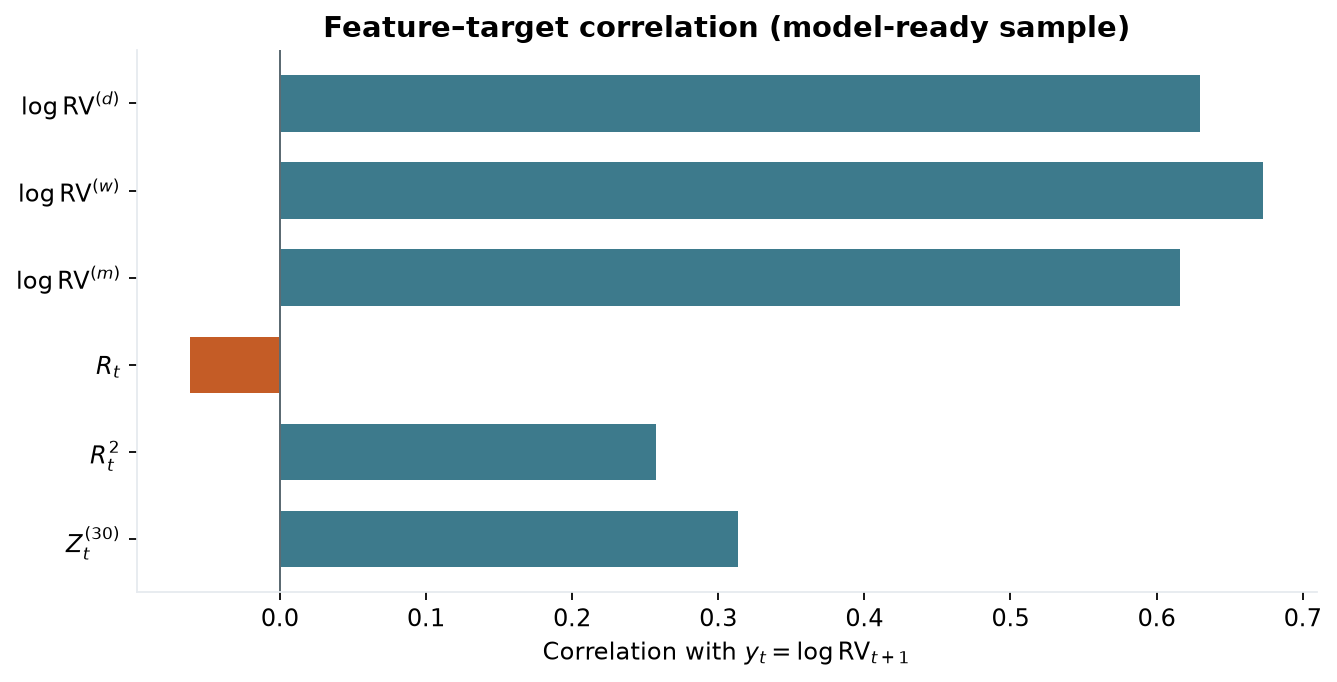
\includegraphics[width=0.92\textwidth]{corr_with_y.png}
\caption{Pearson correlation of panel columns with \(y_t\).}
\end{figure}
\begin{figure}[H]
\centering
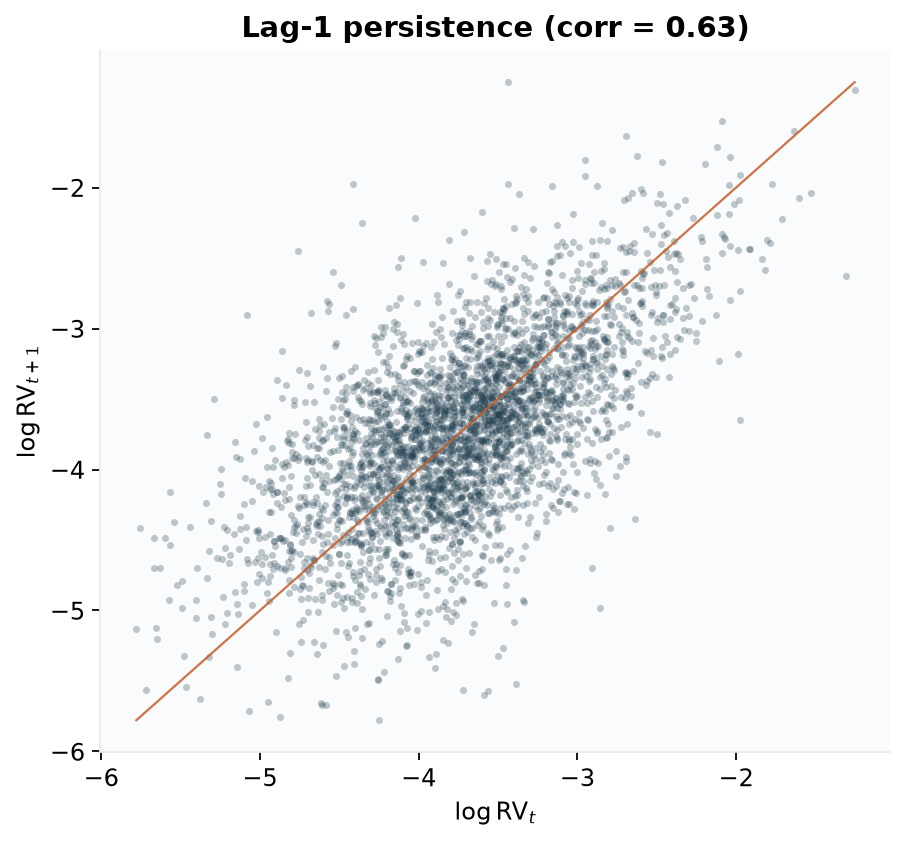
\includegraphics[width=0.72\textwidth]{lag1_scatter.png}
\caption{\(\log\mathrm{RV}_t\) against \(\log\mathrm{RV}_{t+1}\).}
\end{figure}
\begin{explain}
HAR-style log-RV terms dominate (correlations about \(0.62\)--\(0.67\)). Volume \(z\) and \(R_t^2\) are moderate. Signed \(R_t\) is near zero---useful as GARCH's data process, not as a stand-alone predictor of next-day \(\log\mathrm{RV}\).
\end{explain}

\subsection{Collinearity among panel columns}
\begin{figure}[H]
\centering
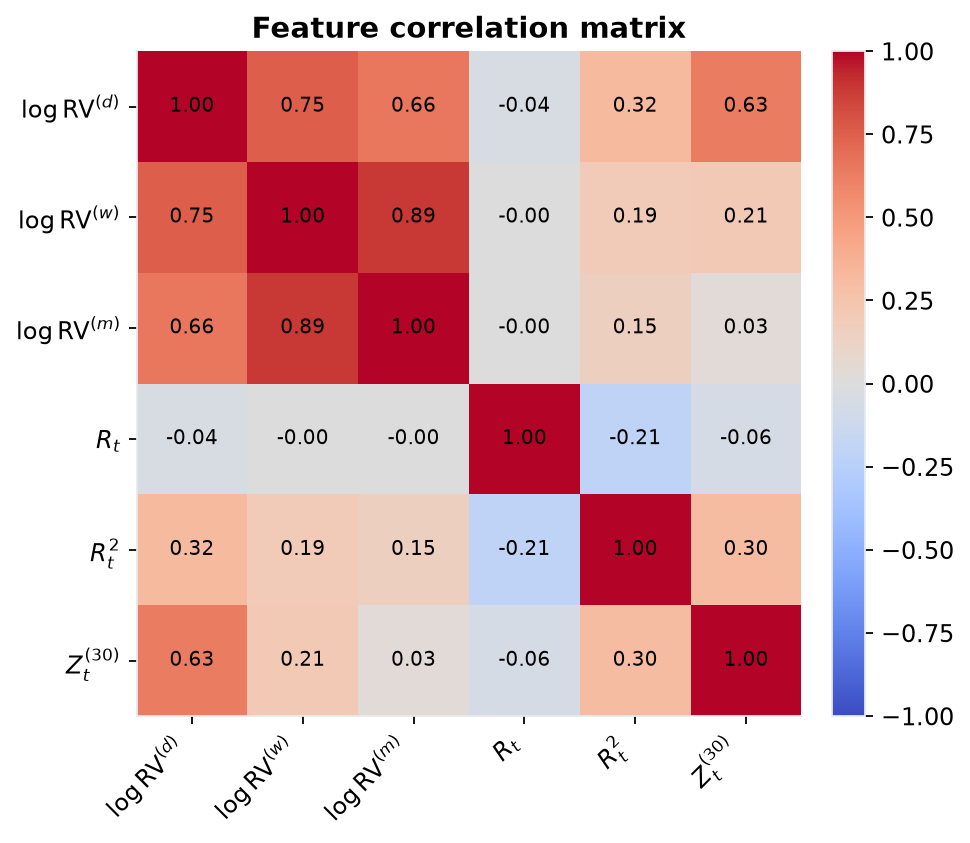
\includegraphics[width=0.78\textwidth]{feature_corr.png}
\caption{Pairwise correlations (red $=$ strong positive, blue $=$ strong negative).}
\end{figure}
\begin{explain}
The large red block among \(\log\mathrm{RV}^{(d)}\), \(\log\mathrm{RV}^{(w)}\), and \(\log\mathrm{RV}^{(m)}\) is expected: the week and month terms are rolling averages of the same series, so they move together by construction (pairwise correlations about \(0.66\)--\(0.89\)). That is not a signal to delete two HAR lags. HAR is designed that way; coefficients are read jointly as a multi-horizon decomposition, not as three independent effects. Signed \(R_t\) is almost uncorrelated with the HAR block. Volume \(z\) moves with daily \(\log\mathrm{RV}\) (about \(0.63\)) but much less with the month term.
\end{explain}

\subsection{Panel columns}
\begin{table}[H]
\centering
\begin{tabular}{llll}
\toprule
Column & Definition & HAR / ARIMA & GARCH / LSTM \\
\midrule
\texttt{log\_rv\_d/w/m} & HAR log-RV terms & HAR uses all three & LSTM window channels \\
\texttt{log\_rv} & daily \(\log\mathrm{RV}_t\) & ARIMA series & LSTM window channel \\
\texttt{ret\_d} & \(R_t\) & --- & GARCH series \\
\texttt{ret\_d\_sq} & \(R_t^2\) & --- & LSTM window channel \\
\texttt{volume\_z30} & volume \(z\) & --- & LSTM window channel \\
\texttt{y} & \(\log\mathrm{RV}_{t+1}\) & target & target \\
\bottomrule
\end{tabular}
\caption{Same parquet panel; different models read different columns.}
\end{table}
\begin{explain}
File: \texttt{data/processed/btcusdt\_1d\_features.parquet}. The LSTM scaler is fit on the fitting sample only (train while tuning; train+val on the final refit).
\end{explain}

\section{Evaluation protocol}
The out-of-sample rules are fixed in \texttt{eval\_freeze/protocol.py} and shared by every model.
No model redefines the splits or the metrics.

\subsection{What is frozen}
\begin{itemize}
  \item Target: \(y_t=\log\mathrm{RV}_{t+1}\)
  \item Chronological train / val / test cuts (no shuffle)
  \item Protocol B: tune, then refit on train+val, score on test
  \item Metrics: RMSE and MAE on log-RV; MAPE and QLIKE on RV
  \item Val usage: LSTM tuning and early stopping only
\end{itemize}
\begin{explain}
The classical series model on \(\log\mathrm{RV}\) is ARIMA. Multi-horizon persistence is handled by HAR.
\end{explain}

\subsection{Chronological splits}
\begin{table}[H]
\centering
\begin{tabular}{llrr}
\toprule
Split & Role & Dates (UTC) & \(n\) \\
\midrule
Train & Tuning-stage fit & 17 Sep 2017 -- 31 Dec 2021 & 1{,}540 \\
Val & LSTM tune / early stop only & 1 Jan 2022 -- 31 Dec 2023 & 729 \\
Train+Val & Final fit before test & 17 Sep 2017 -- 31 Dec 2023 & 2{,}269 \\
Test & Reported scores only & 1 Jan 2024 -- 25 Sep 2026 & 999 \\
\bottomrule
\end{tabular}
\caption{Frozen calendar.}
\end{table}
\begin{figure}[H]
\centering
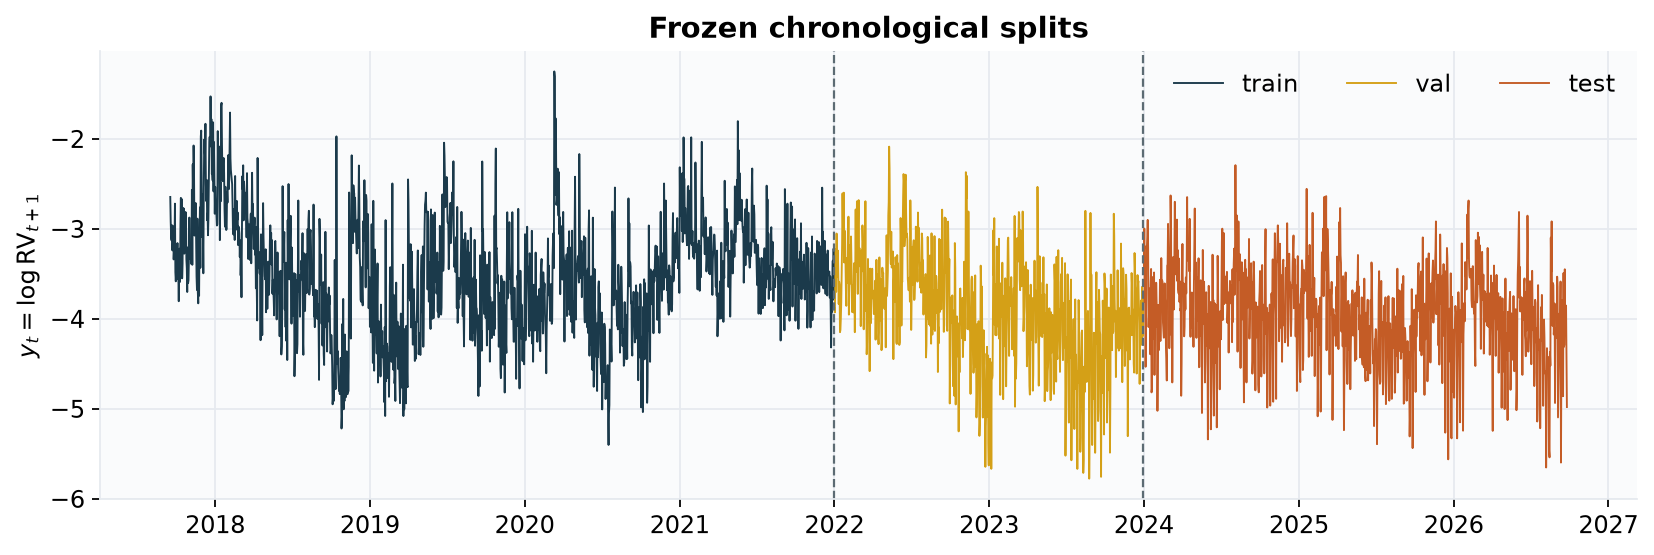
\includegraphics[width=\textwidth]{splits_timeline.png}
\caption{Target path colored by split.}
\end{figure}
\begin{explain}
Workflow: (1) tune on train, using val for the LSTM only; (2) refit on train+val with frozen choices; (3) score on test.
\end{explain}

\subsection{Metrics}
\[
\mathrm{RMSE}=\sqrt{\frac1n\sum (y_t-\hat y_t)^2},
\qquad
\mathrm{MAE}=\frac1n\sum |y_t-\hat y_t|,
\]
\[
\mathrm{MAPE}
=
\frac{100}{n}\sum_t
\frac{\bigl|\widehat{\mathrm{RV}}_{t+1}-\mathrm{RV}_{t+1}\bigr|}{\mathrm{RV}_{t+1}},
\qquad
\mathrm{QLIKE}
=
\frac1n\sum_t
\Biggl(
\frac{\mathrm{RV}_{t+1}}{\widehat{\mathrm{RV}}_{t+1}}
-
\ln\frac{\mathrm{RV}_{t+1}}{\widehat{\mathrm{RV}}_{t+1}}
-1
\Biggr).
\]
\begin{explain}
RMSE and MAE use the log-RV scale. MAPE and QLIKE use \(\widehat{\mathrm{RV}}=\exp(\hat y)\) for log-RV models, and GARCH \(\hat\sigma\) for the GARCH forecast. AIC is used only to pick ARIMA and GARCH orders on train. It is not a test score.
\end{explain}

\subsection{Sanity check}
A parameter-free lag-1 rule \(\hat y_t=\log\mathrm{RV}_t\) checks that the splits and metric code run. The same rule is the Naive baseline in the next section.
\begin{figure}[H]
\centering
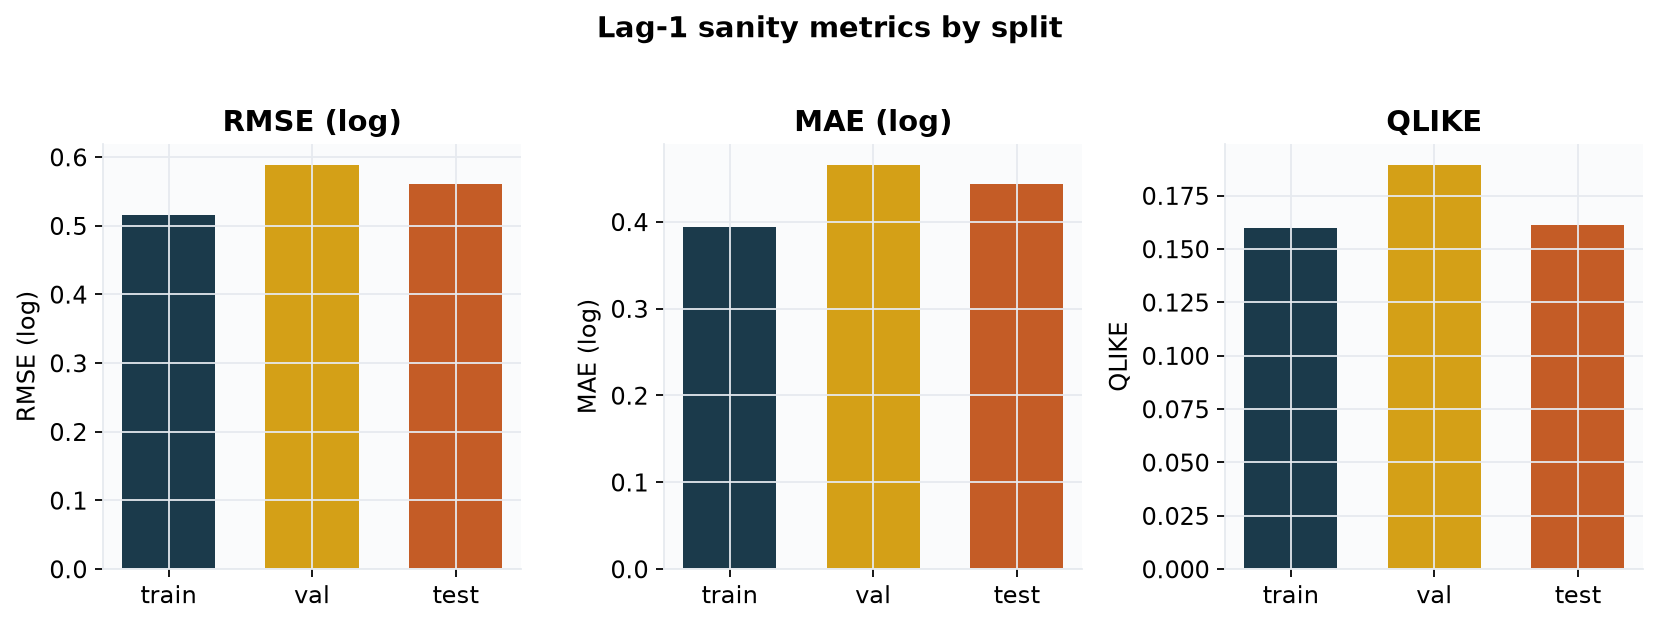
\includegraphics[width=\textwidth]{naive_metrics.png}
\caption{Lag-1 metrics by split.}
\end{figure}
\begin{table}[H]
\centering
\begin{tabular}{lccc}
\toprule
Split & RMSE (log) & MAE (log) & QLIKE \\
\midrule
Train & 0.516 & 0.394 & 0.160 \\
Val & 0.589 & 0.466 & 0.190 \\
Test & 0.560 & 0.444 & 0.161 \\
\bottomrule
\end{tabular}
\caption{Lag-1 scores on each split.}
\end{table}

\section{Classical baselines}
Naive, GARCH, ARIMA, and HAR under Protocol~B.
Script: \texttt{models/run\_baselines.py}.
Tune on train (AIC where needed), final fit on train+val, score on test
(2024-01-01 through 2026-09-25, \(n=999\)).
GARCH is scored once against Naive, then left out of the realized-volatility ladder.

\subsection{Naive}
\[
\hat y_t=\log\mathrm{RV}_t.
\]
\begin{explain}
No parameters. Test RMSE \(0.560\), MAE \(0.444\), MAPE \(51.1\%\), QLIKE \(0.161\). Reference forecast for the ladder.
\end{explain}

\subsection{GARCH}
AIC on train over \(\{(1,1),(1,2),(2,1)\}\) selected GARCH\((2,1)\) on daily returns (percent scale).
Parameters refit on train+val; one-step \(\hat\sigma_{t+1}\) walked forward on the return path with frozen coefficients.
Scored against realized \(\mathrm{RV}_{t+1}\) / \(\log\mathrm{RV}_{t+1}\).

\begin{table}[H]
\centering
\begin{tabular}{lcccc}
\toprule
Model & RMSE (log) & MAE (log) & MAPE (\%) & QLIKE \\
\midrule
Naive & \textbf{0.560} & \textbf{0.444} & \textbf{51.1} & 0.161 \\
GARCH\((2,1)\) & 0.656 & 0.523 & 82.9 & 0.161 \\
\bottomrule
\end{tabular}
\caption{GARCH vs Naive on the test window. Bold marks the better score; QLIKE is tied at the reported precision.}
\end{table}
\begin{explain}
GARCH forecasts conditional return volatility: how large tomorrow's daily return is expected to be, given past returns.
The target of this study is intraday realized volatility: how much the price wiggled during day \(t+1\).
Those are related objects, not the same reading. Scored against \(\mathrm{RV}_{t+1}\), GARCH trails lag-1 Naive on RMSE, MAE, and MAPE, and matches it on QLIKE.
That is an object mismatch, not evidence that GARCH is a failed return model.
GARCH therefore leaves the RV race. The remaining classical models are ARIMA and HAR.
\end{explain}

\subsection{ARIMA}
Order selected by AIC on train: ARIMA\((3,0,3)\). Refit on train+val; one-step forecasts on test with frozen parameters (state updated by appending realized \(\log\mathrm{RV}\)).
\begin{explain}
Beats Naive (RMSE \(0.518\), MAE \(0.407\), MAPE \(47.4\%\), QLIKE \(0.132\)) and trails HAR below. A generic ARMA on \(\log\mathrm{RV}\) is the next step before the structured multi-horizon model.
\end{explain}

\subsection{HAR}
Following Corsi~\cite{corsi2009}, next-day \(\log\mathrm{RV}\) is regressed on daily, weekly, and monthly components:
\[
\hat y_t
=
\hat c
+ \hat\beta_d\log\mathrm{RV}^{(d)}_t
+ \hat\beta_w\log\mathrm{RV}^{(w)}_t
+ \hat\beta_m\log\mathrm{RV}^{(m)}_t.
\]
OLS on train+val (\(n=2269\)):
\(\hat c=-0.341\), \(\hat\beta_d=0.299\), \(\hat\beta_w=0.457\), \(\hat\beta_m=0.151\).
\begin{explain}
Weekly component carries the largest weight. Test RMSE \(0.458\), MAE \(0.354\), MAPE \(40.7\%\), QLIKE \(0.101\). Best classical score on the RV ladder: structured day/week/month lags beat the ARIMA above.
\end{explain}

\subsection{Classical test scores}
\begin{table}[H]
\centering
\begin{tabular}{lcccc}
\toprule
Model & RMSE (log) & MAE (log) & MAPE (\%) & QLIKE \\
\midrule
Naive & 0.560 & 0.444 & 51.1 & 0.161 \\
ARIMA\((3,0,3)\) & 0.518 & 0.407 & 47.4 & 0.132 \\
HAR & \textbf{0.458} & \textbf{0.354} & \textbf{40.7} & \textbf{0.101} \\
\bottomrule
\end{tabular}
\caption{Test metrics on the RV ladder. Bold marks the best classical score in each column. GARCH was scored above and is not on this board.}
\end{table}
\begin{figure}[H]
\centering
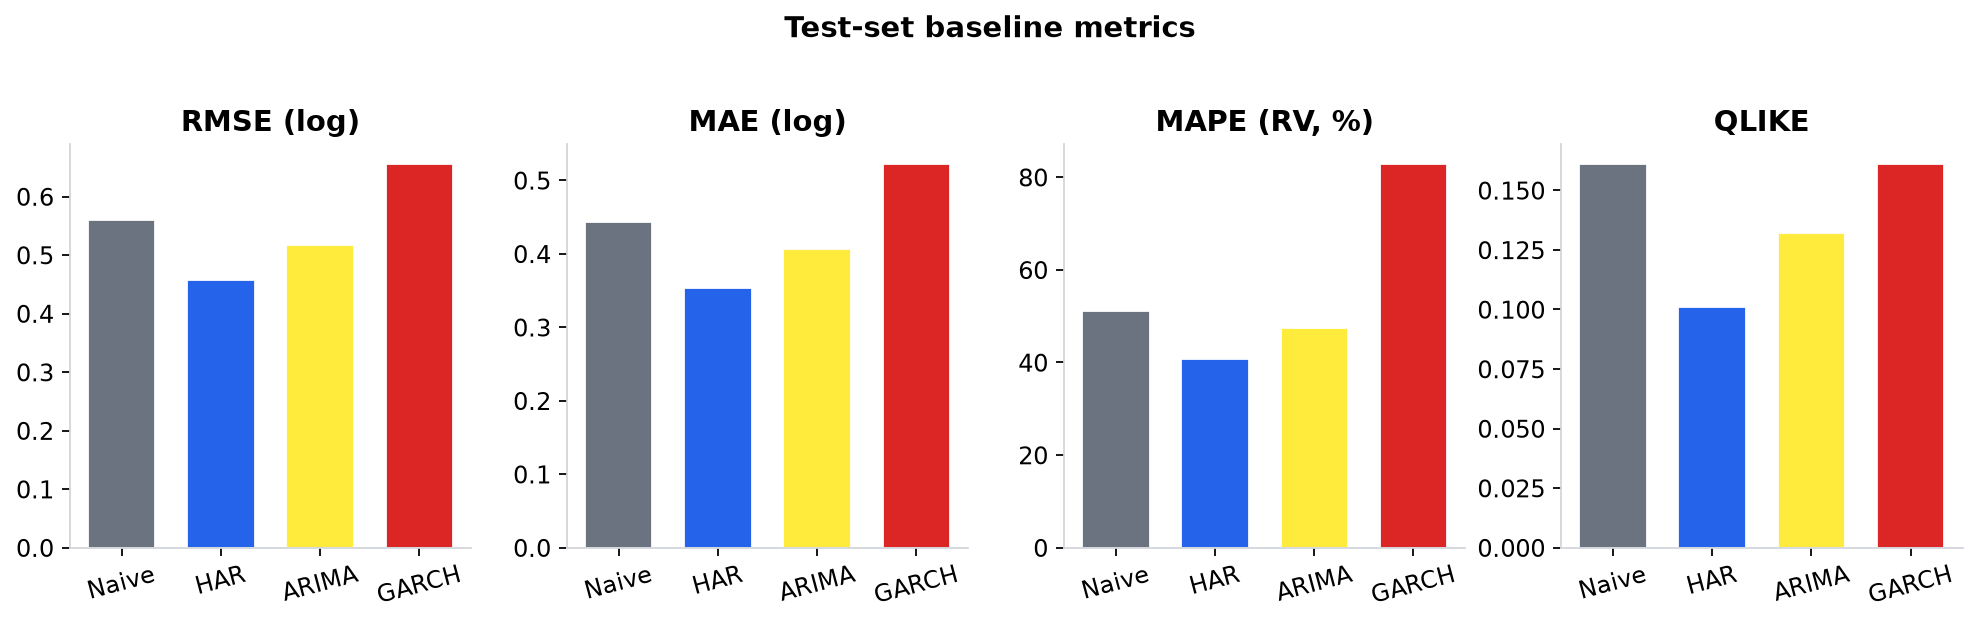
\includegraphics[width=\textwidth]{baseline_metrics.png}
\caption{Test metrics by model on the RV ladder.}
\end{figure}
\begin{figure}[H]
\centering
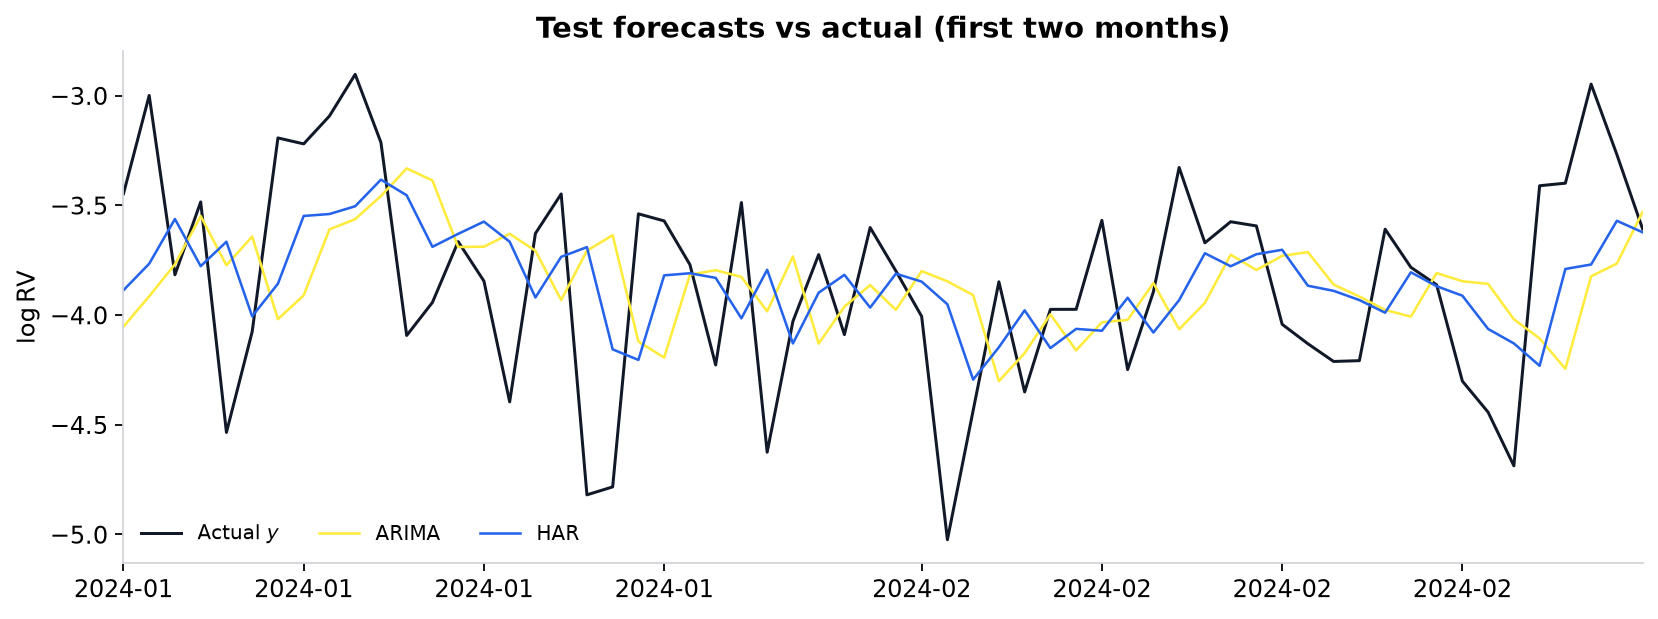
\includegraphics[width=\textwidth]{baseline_test_paths_2mo.png}
\caption{Test path, first two months (2024-01 through 2024-02).}
\end{figure}
\begin{figure}[H]
\centering
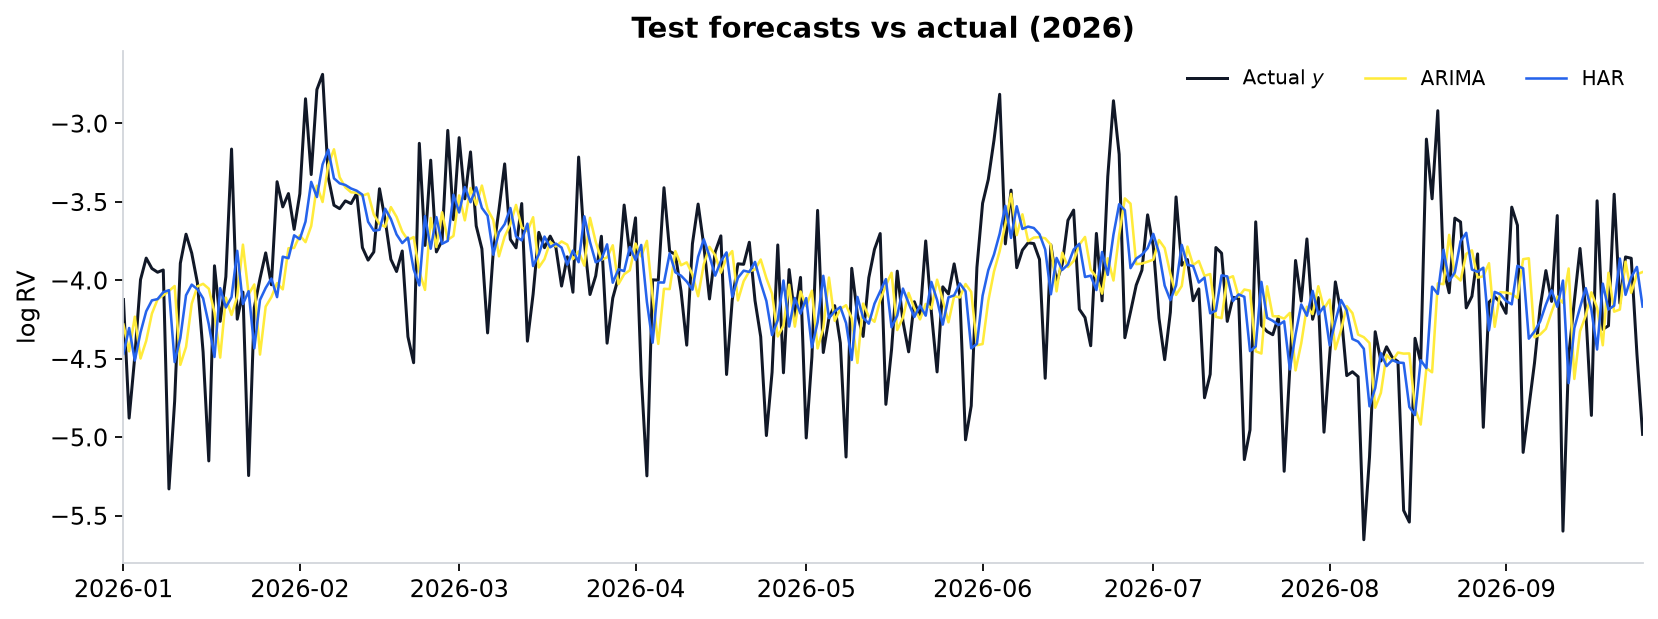
\includegraphics[width=\textwidth]{baseline_test_paths.png}
\caption{Test path in calendar 2026.}
\end{figure}
\begin{explain}
Among the RV models, HAR has the lowest test error. ARIMA improves on Naive and trails HAR.
\end{explain}

\section{Recurrent networks and LSTMs}
Recurrent neural networks (RNNs) and long short-term memory (LSTM) cells process
sequences by carrying a state across time~\cite{goodfellow2016}.
This section states the recurrence, the training failure modes of a plain RNN,
and the gated LSTM update used for one-day-ahead \(\log\mathrm{RV}\) forecasting.

\subsection{Why recurrence}
A feed-forward net maps one input vector to one output.
A time series needs something else: the prediction at step \(t\) should depend on
what came before, not only on \(x_t\).

An RNN does that with a \emph{hidden state} \(h_t\) that is updated every step and
passed forward. The same parameters are reused at every \(t\).
In compact form,
\[
\hat y_t \;=\; f\!\bigl(x_t,\, h_{t-1}\bigr).
\]
\begin{figure}[H]
\centering
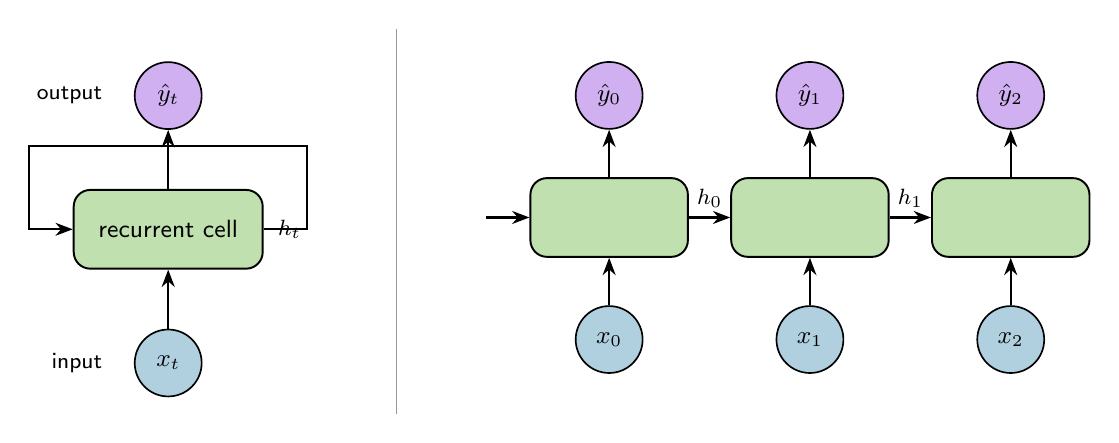
\begin{tikzpicture}[
  cell/.style={draw=black, fill=MITgreen, rounded corners=6pt,
               minimum width=2.4cm, minimum height=1.0cm,
               font=\sffamily\small, align=center, line width=0.7pt},
  ycirc/.style={circle, draw=black, fill=MITpurple, minimum size=0.85cm,
               inner sep=0pt, font=\small, line width=0.6pt},
  xcirc/.style={circle, draw=black, fill=MITblue, minimum size=0.85cm,
               inner sep=0pt, font=\small, line width=0.6pt},
  arr/.style={-{Stealth[length=2.2mm]}, line width=0.75pt, black},
  ]
  \begin{scope}[shift={(0,0)}]
    \node[cell] (cellL) {recurrent cell};
    \node[ycirc, above=0.75cm of cellL] (yL) {$\hat{y}_t$};
    \node[xcirc, below=0.75cm of cellL] (xL) {$x_t$};
    \draw[arr] (cellL.north) -- (yL.south);
    \draw[arr] (xL.north) -- (cellL.south);
    \node[left=0.28cm of yL, font=\sffamily\footnotesize, anchor=east] {output};
    \node[left=0.28cm of xL, font=\sffamily\footnotesize, anchor=east] {input};
    \coordinate (rA) at ([xshift=0.55cm]cellL.east);
    \coordinate (rB) at ([xshift=0.55cm,yshift=0.55cm]cellL.north east);
    \coordinate (rC) at ([xshift=-0.55cm,yshift=0.55cm]cellL.north west);
    \coordinate (rD) at ([xshift=-0.55cm]cellL.west);
    \draw[line width=0.75pt, black, -{Stealth[length=2.2mm]}]
      (cellL.east) -- (rA) -- (rB) -- (rC) -- (rD) -- (cellL.west);
    \node[font=\footnotesize, anchor=west] at ([xshift=0.06cm]cellL.east) {$h_t$};
  \end{scope}
  \draw[black!40, line width=0.6pt] (2.9,-2.35) -- (2.9,2.55);
  \begin{scope}[shift={(5.6,0.15)}]
    \foreach \i/\labx/\laby in {0/$x_0$/$\hat{y}_0$, 1/$x_1$/$\hat{y}_1$, 2/$x_2$/$\hat{y}_2$} {
      \pgfmathsetmacro{\xpos}{\i*2.55}
      \node[cell, minimum width=2.0cm] (C\i) at (\xpos,0) {};
      \node[ycirc] (Y\i) at (\xpos,1.55) {\laby};
      \node[xcirc] (X\i) at (\xpos,-1.55) {\labx};
      \draw[arr] (C\i.north) -- (Y\i.south);
      \draw[arr] (X\i.north) -- (C\i.south);
    }
    \draw[arr] (C0.east) -- node[above, font=\footnotesize, pos=0.5] {$h_0$} (C1.west);
    \draw[arr] (C1.east) -- node[above, font=\footnotesize, pos=0.5] {$h_1$} (C2.west);
    \draw[arr] ([xshift=-0.55cm]C0.west) -- (C0.west);
  \end{scope}
\end{tikzpicture}
\caption{Recurrent cell (left) and the same recurrence over three time steps (right).}
\end{figure}

\subsection{A simple RNN cell}
The simplest recurrent unit applies one nonlinearity to the concatenated
current input and previous hidden state:
\[
h_t \;=\; \tanh\!\bigl(W\,[h_{t-1},\, x_t] + b\bigr).
\]
Everything that the network ``remembers'' must travel through that single path.
\begin{figure}[H]
\centering
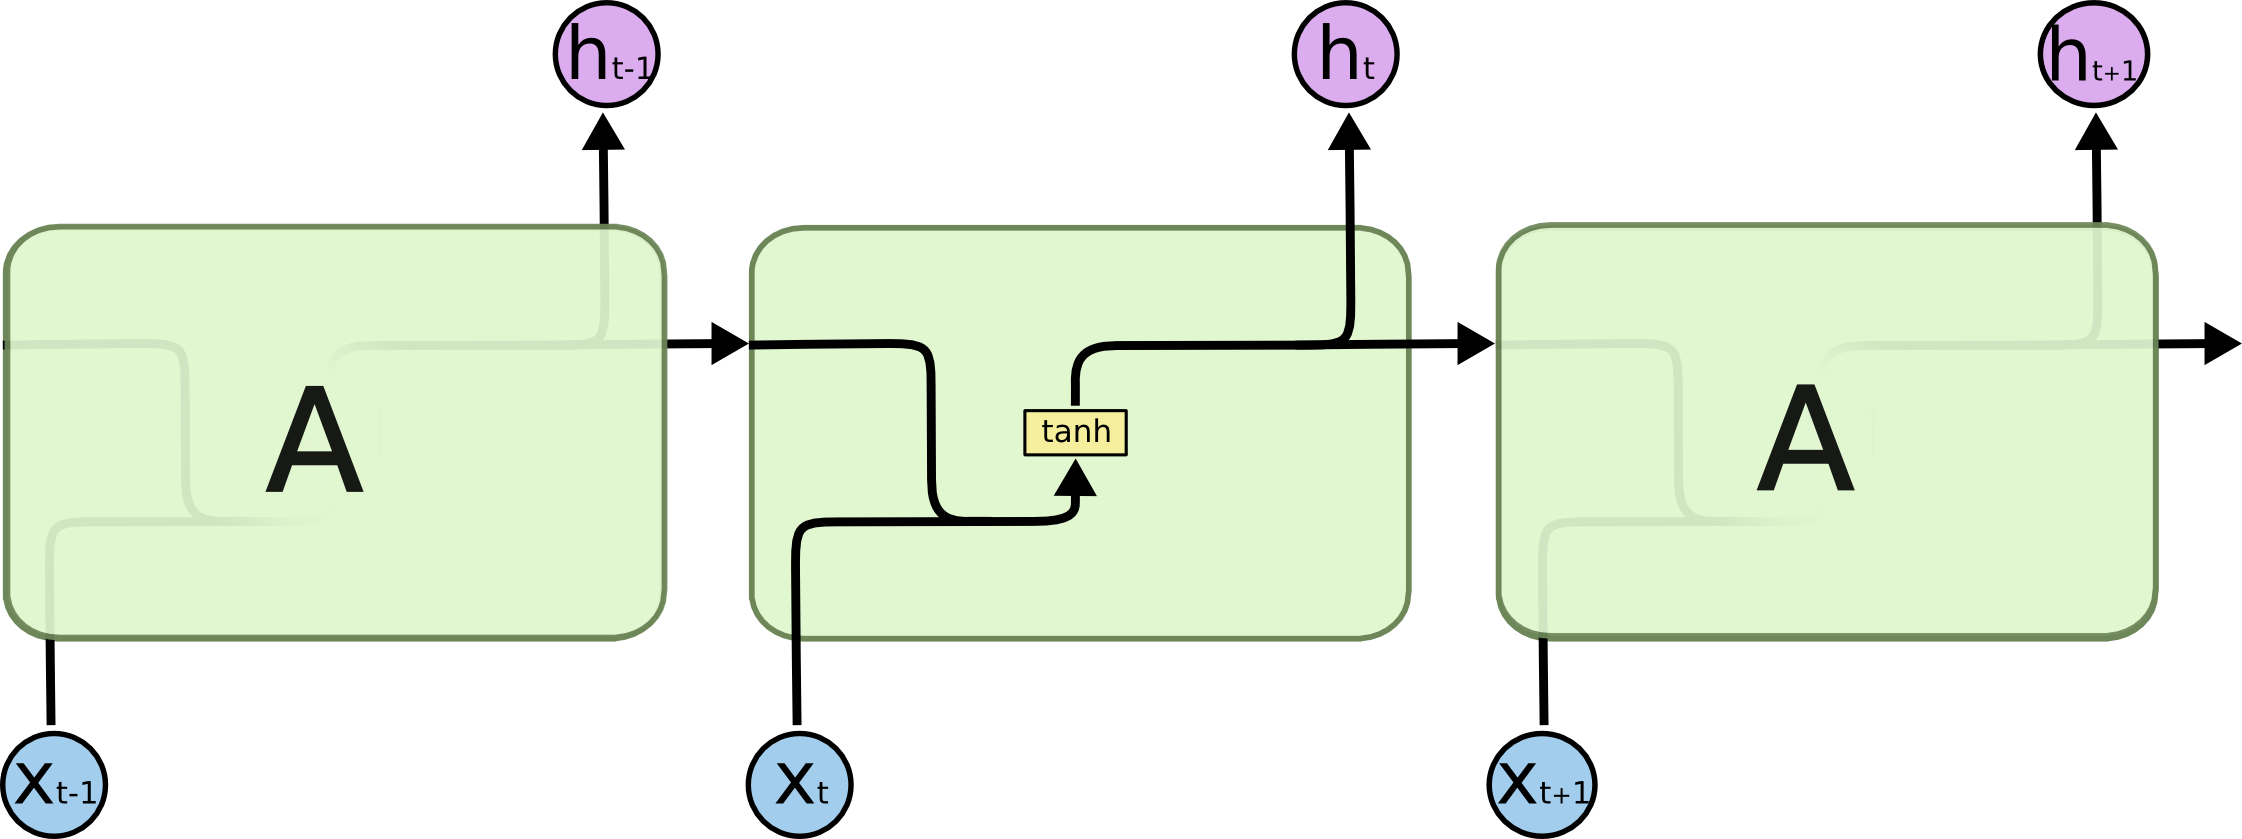
\includegraphics[width=0.92\textwidth]{LSTM3-SimpleRNN.png}
\caption{Repeating RNN module~\cite{olah2015}. Inside \(A\): one \(\tanh\) layer.
\(h_t\) is both the output at \(t\) and the memory passed to \(t+1\).}
\end{figure}

\subsection{Problems of a plain RNN}
Training unrolls the recurrence over many steps (backpropagation through time).
The same weights are applied at every \(t\), so gradients are products of many
Jacobians. Two failure modes follow.

\noindent\textbf{Exploding gradients.}
If those products grow without bound, updates become unstable.
A standard fix is \emph{gradient clipping}~\cite{goodfellow2016}: after the backward pass, shrink the
gradient vector when its norm exceeds a threshold \(\tau\).

\begin{algorithm}[H]
\caption{Algorithm. Gradient clipping}
\begin{algorithmic}
\State \(\mathbf{g} \gets \nabla_{\theta}\mathcal{L}\)
\If{\(\lVert\mathbf{g}\rVert > \tau\)}
  \State \(\mathbf{g} \gets \tau\,\mathbf{g}/\lVert\mathbf{g}\rVert\)
\EndIf
\State \(\theta \gets \theta - \eta\,\mathbf{g}\)
\end{algorithmic}
\end{algorithm}

Clipping controls the size of the step. It does not create a better path for
information to travel across time.

\noindent\textbf{Vanishing gradients.}
If the products shrink toward zero, early timesteps stop affecting the loss.
Weight updates then ignore long-range dependence even when it is present in the
data. Rescaling \(\mathbf{g}\) does not fix that: the signal from the distant past
is already gone. The usual remedy is architectural---a cell that can carry
state across many steps without repeatedly multiplying through a saturating
nonlinearity. That motivates the LSTM below.

\subsection{LSTM: a gated memory}
An LSTM keeps two signals at each step:
\begin{itemize}
  \item a \emph{cell state} \(c_t\) --- a slow path that can carry information across many steps with mostly linear updates;
  \item a \emph{hidden state} \(h_t\) --- the exposed summary used as output and as input to the next step.
\end{itemize}
Three sigmoid \emph{gates} (values in \((0,1)\)) control write / erase / read on the cell.
\begin{figure}[H]
\centering
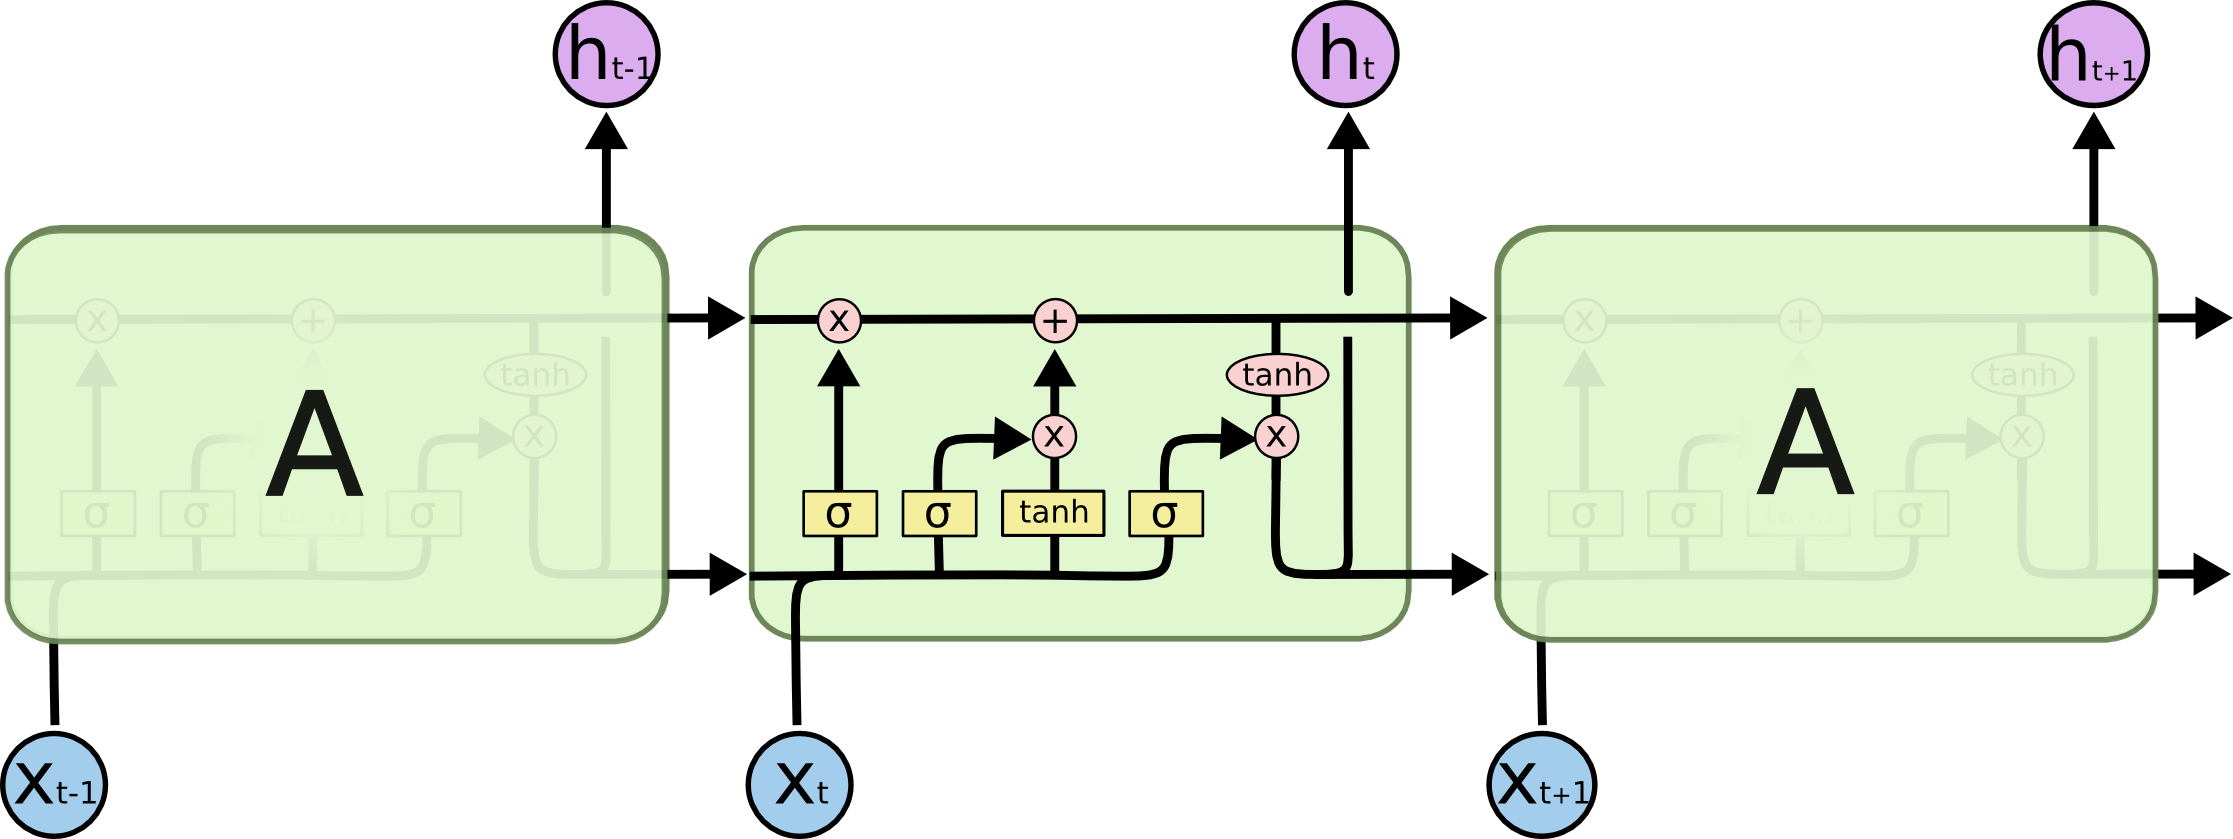
\includegraphics[width=0.95\textwidth]{LSTM3-chain.png}\\[0.8em]
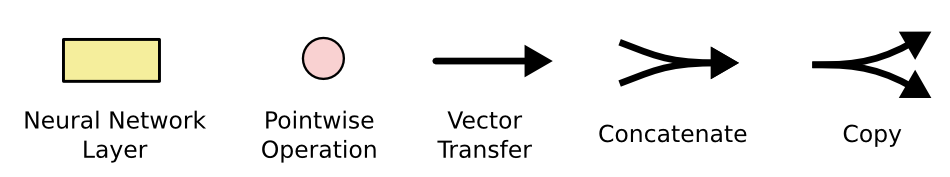
\includegraphics[width=0.72\textwidth]{LSTM2-notation.png}
\caption{LSTM chain~\cite{olah2015}. The top horizontal line is the cell state.
Gates (yellow \(\sigma\) / \(\tanh\) layers and pink pointwise ops) edit that line
at each step, then form \(h_t\).}
\end{figure}

\subsection{Gates, step by step}
On timestep \(t\), the network receives \(x^{(t)}\) and the previous pair
\(\bigl(h^{(t-1)},\, c^{(t-1)}\bigr)\), and produces
\(\bigl(h^{(t)},\, c^{(t)}\bigr)\):
\begin{align*}
\bm{f}^{(t)}
  &= \sigma\!\bigl(W_f\,\bm{h}^{(t-1)} + U_f\,\bm{x}^{(t)} + \bm{b}_f\bigr)
  && \text{forget gate} \\[4pt]
\bm{i}^{(t)}
  &= \sigma\!\bigl(W_i\,\bm{h}^{(t-1)} + U_i\,\bm{x}^{(t)} + \bm{b}_i\bigr)
  && \text{input gate} \\[4pt]
\bm{o}^{(t)}
  &= \sigma\!\bigl(W_o\,\bm{h}^{(t-1)} + U_o\,\bm{x}^{(t)} + \bm{b}_o\bigr)
  && \text{output gate} \\[4pt]
\tilde{\bm{c}}^{(t)}
  &= \tanh\!\bigl(W_c\,\bm{h}^{(t-1)} + U_c\,\bm{x}^{(t)} + \bm{b}_c\bigr)
  && \text{candidate content} \\[4pt]
\bm{c}^{(t)}
  &= \bm{f}^{(t)}\odot \bm{c}^{(t-1)} + \bm{i}^{(t)}\odot \tilde{\bm{c}}^{(t)}
  && \text{cell update} \\[4pt]
\bm{h}^{(t)}
  &= \bm{o}^{(t)}\odot \tanh\bm{c}^{(t)}
  && \text{hidden state}
\end{align*}

Forget scales the old cell (near \(0\) erases, near \(1\) keeps).
Input scales how much new candidate content is written.
Output chooses what of \(\tanh(c_t)\) becomes \(h_t\).
The cell update is almost additive: erase some of \(c_{t-1}\), add some of \(\tilde c_t\).
That additive path is what makes long-range gradients viable.

\begin{figure}[H]
\centering
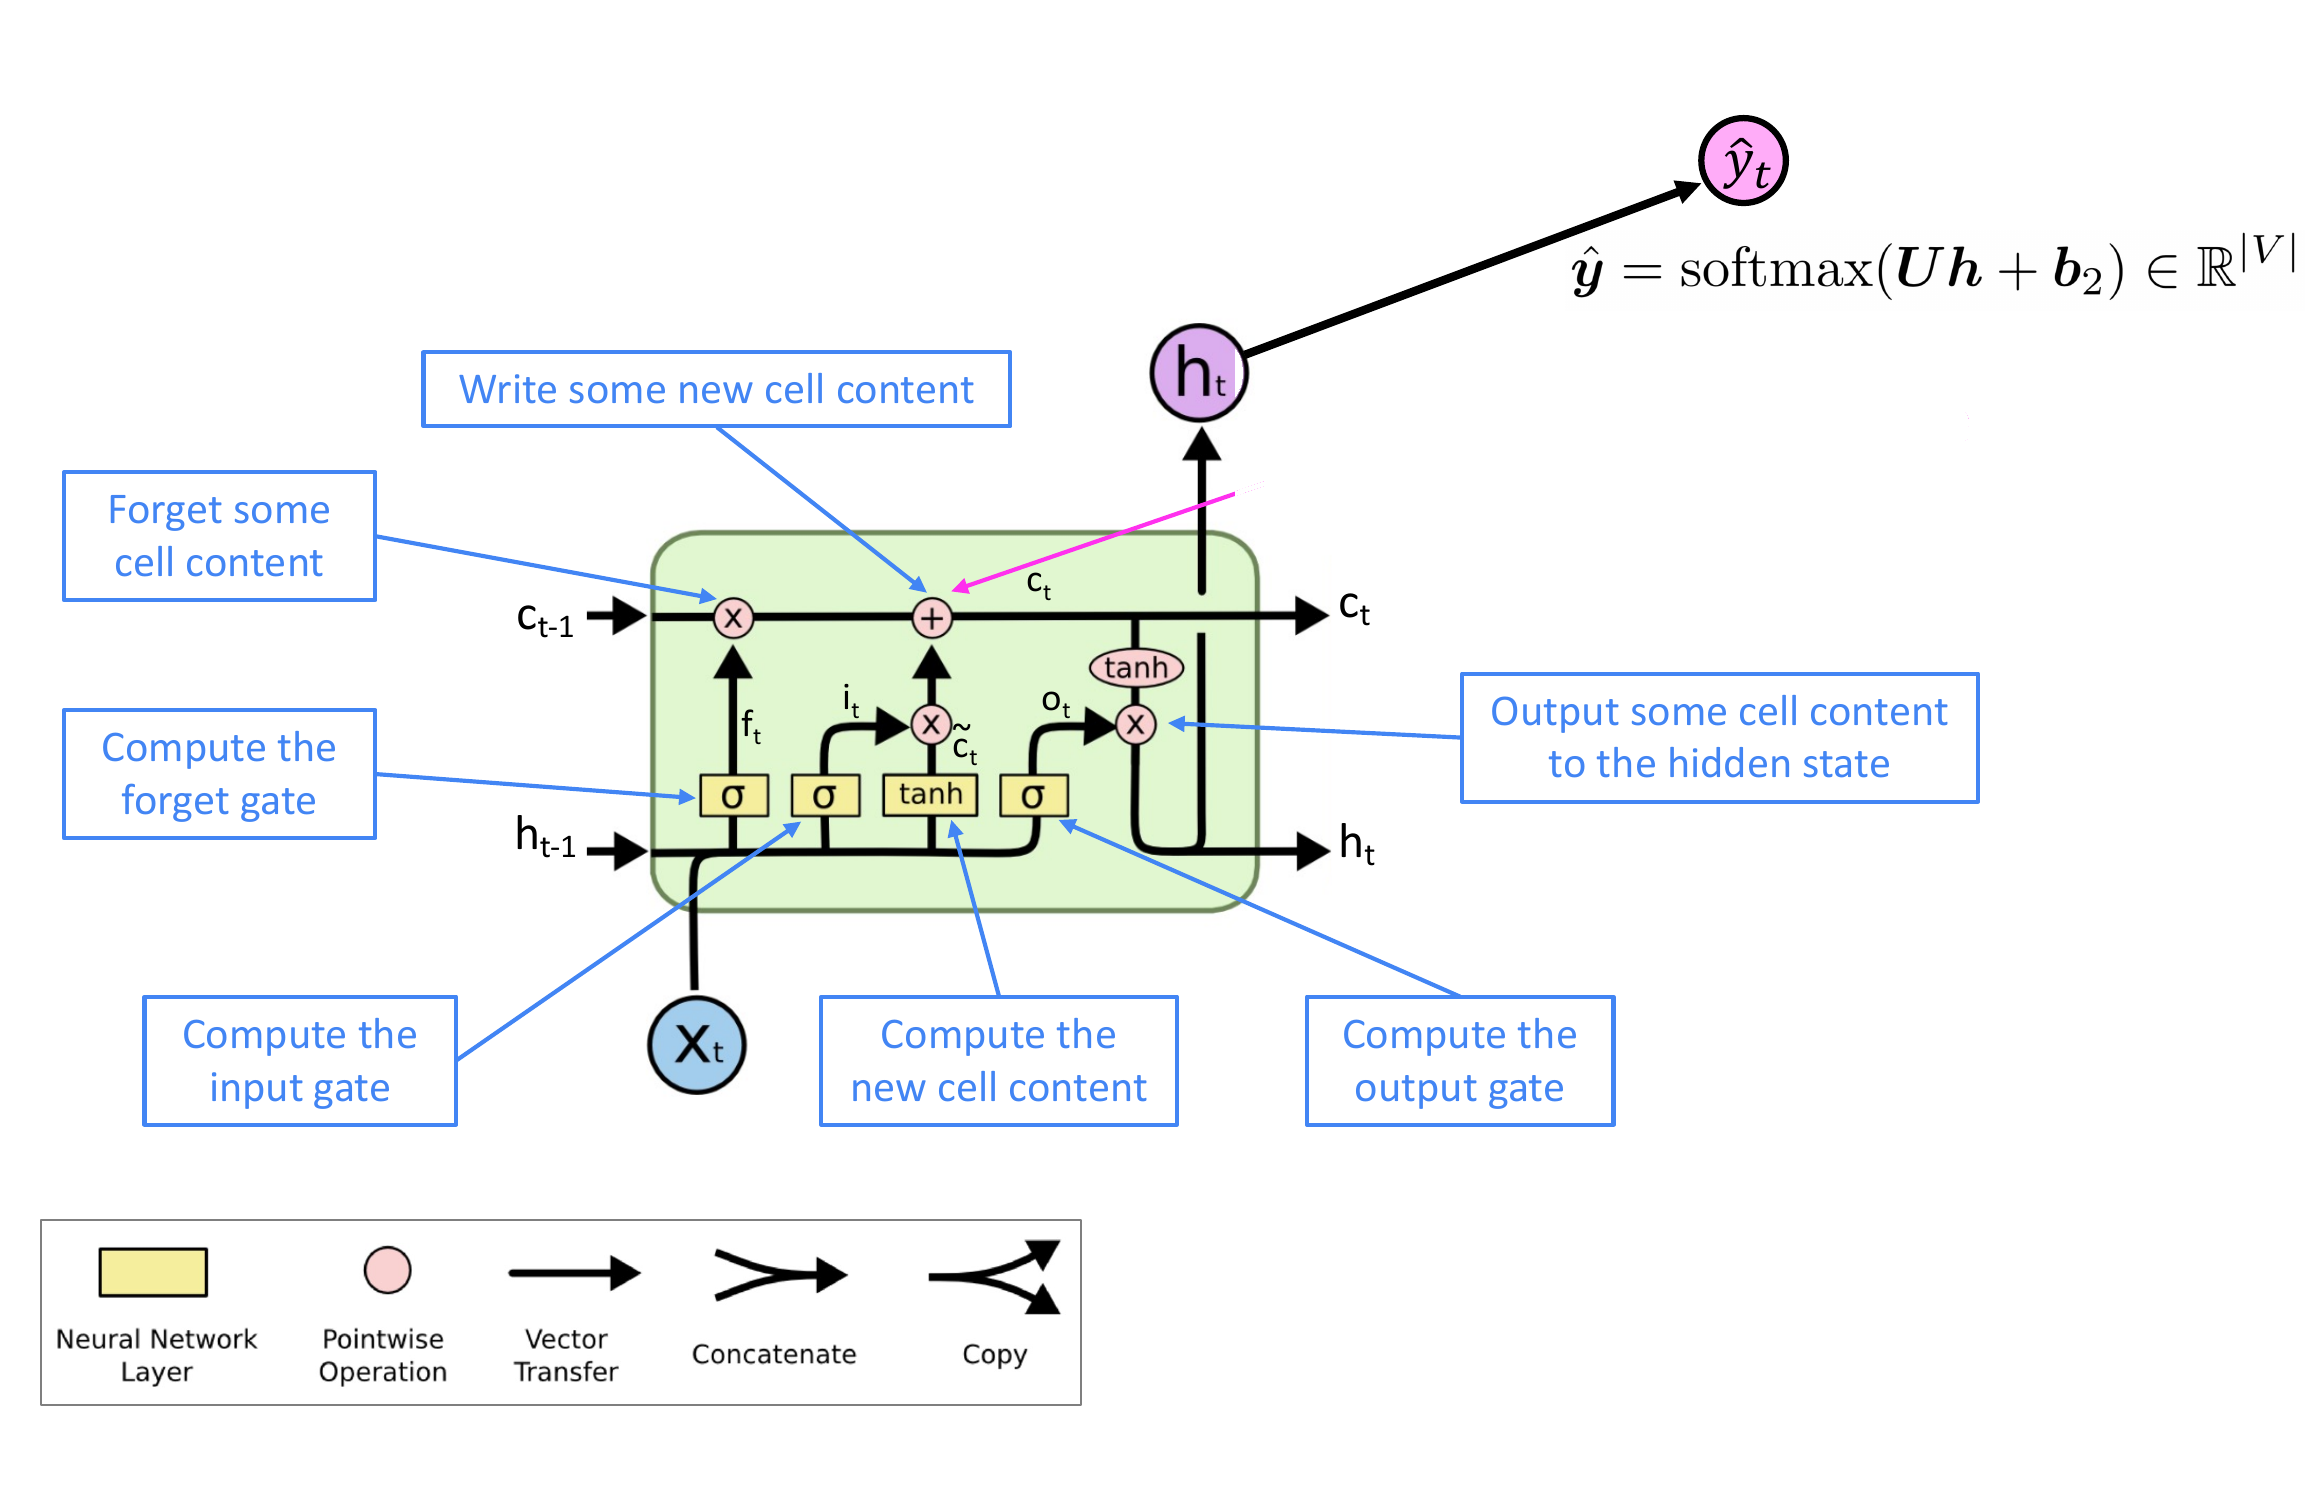
\includegraphics[width=0.98\textwidth]{Stanford-CS224N-L6-slide24.png}
\caption{Annotated LSTM cell: forget, write, and read
on the cell state, then \(h_t\) (and an optional readout \(\hat y_t\)).}
\end{figure}

\subsection{Reading the cell diagram}
\begin{center}
\renewcommand{\arraystretch}{1.25}
\begin{tabular}{@{}ll@{}}
\hline
\textbf{Signal} & \textbf{Role} \\
\hline
Forget gate \(f_t\) &
  what to keep from \(c_{t-1}\) \\
Input gate \(i_t\) &
  what of \(\tilde c_t\) to write \\
Candidate \(\tilde c_t\) &
  new content proposed at \(t\) \\
Cell \(c_t\) &
  memory: forget then write \\
Output gate \(o_t\) &
  what of the cell to expose \\
Hidden \(h_t\) &
  output at \(t\); input to step \(t+1\) \\
\hline
\end{tabular}
\end{center}
\vspace{0.6em}

In a forecasting model the readout from \(h_t\) is usually a linear map to a scalar
(or a small head), not a softmax over a vocabulary.
The cell mechanics above are unchanged; only the final layer depends on the task.
The next section applies this architecture under the frozen protocol.

\section{LSTM forecast}
Standalone LSTM under the same protocol. The forecast is the network output.
Script: \texttt{models/run\_lstm.py}.

\subsection{Setup}
\begin{itemize}
  \item Target: \(y_t=\log\mathrm{RV}_{t+1}\).
  \item Input window: \(\log\mathrm{RV}\), its 7-day mean, its 22-day mean, squared daily return, and volume \(z\)-score.
  \item Scaler: per-channel mean and standard deviation, fit on the fitting sample only
    (train while tuning; train+val on the final refit).
  \item Optimizer: Adam. Loss: MSE on \(\log\mathrm{RV}\).
  \item Val (2022--2023): grid and early stopping. Test is not used for tuning.
\end{itemize}

\subsection{Hyperparameter grid}
\[
L\in\{22,60\},\quad
h\in\{64,128\},\quad
\mathrm{depth}\in\{1,2\},\quad
\mathrm{dropout}=0.1,\quad
\mathrm{LR}\in\{10^{-3},\,3\cdot 10^{-4}\}.
\]
Sixteen configurations. Each is trained on the training window with early stopping on validation RMSE
(patience 10, maximum 80 epochs). The selected configuration is refit on train+val for the chosen epoch budget.

\begin{figure}[H]
\centering
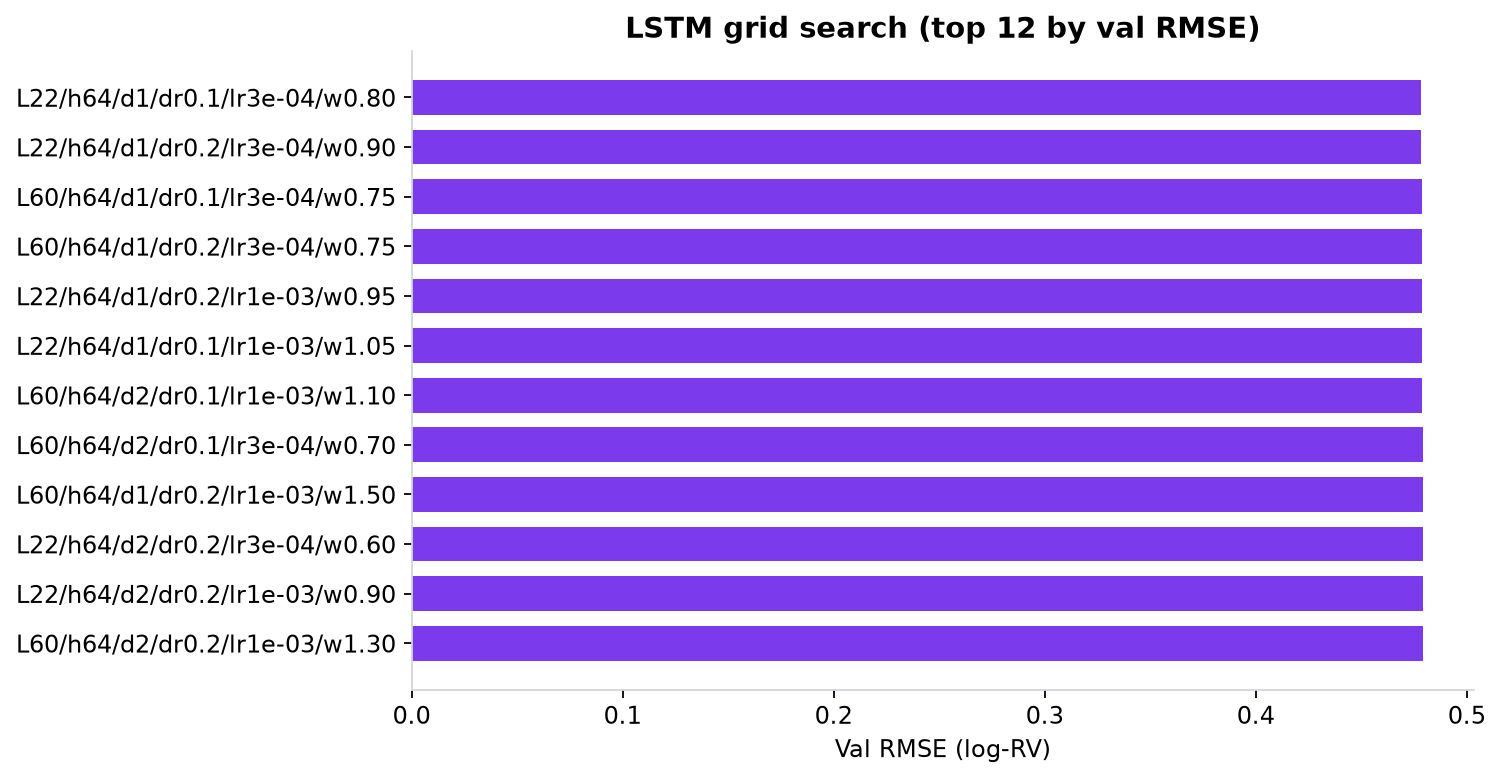
\includegraphics[width=\textwidth]{lstm_val_grid.png}
\caption{Top 12 grid configs by validation RMSE.}
\end{figure}

\begin{figure}[H]
\centering
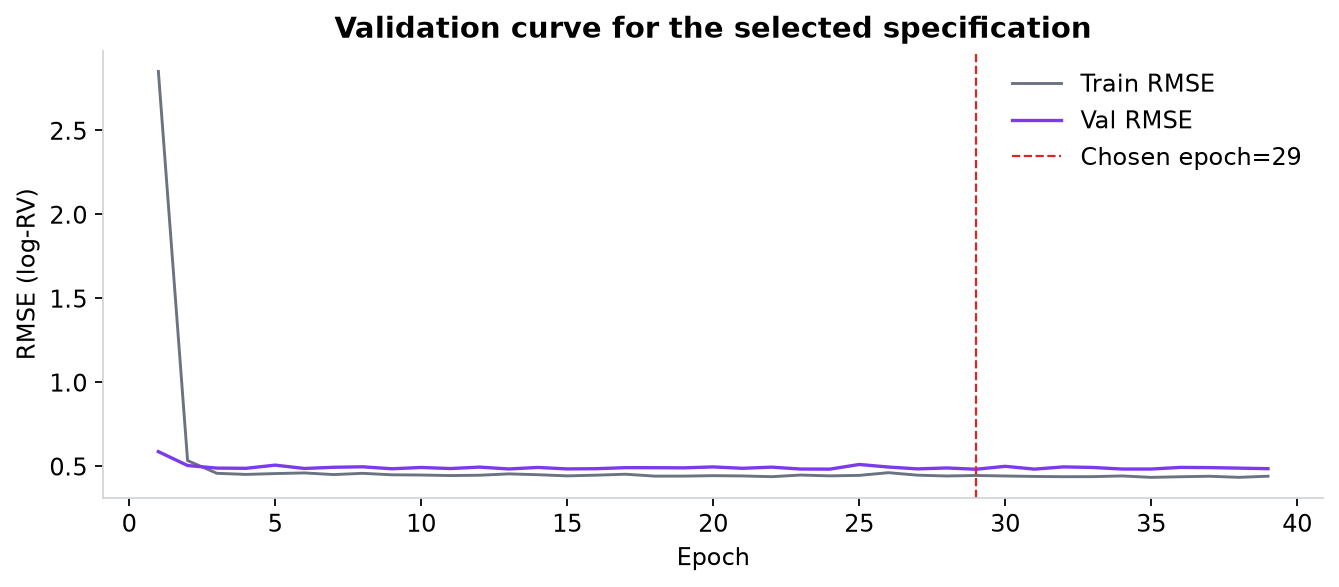
\includegraphics[width=0.95\textwidth]{lstm_learning_curve.png}
\caption{Train vs val RMSE for the winning config; red line = chosen epoch.}
\end{figure}

\subsection{Selected model}
\begin{table}[H]
\centering
\begin{tabular}{lr}
\toprule
Setting & Value \\
\midrule
\(L\) (lookback) & 60 \\
Hidden size & 128 \\
Depth & 1 \\
Dropout & 0.1 \\
Learning rate & \(10^{-3}\) (Adam) \\
Best val epoch & 29 \\
Val RMSE & 0.482 \\
\bottomrule
\end{tabular}
\caption{Winning hyperparameters from the validation grid.}
\end{table}
\begin{explain}
Refit on train+val for 29 epochs with the validation-selected settings, then score the test window once.
\end{explain}

\subsection{Test results}
\(n=999\) (2024-01-01 through 2026-09-25). Naive and HAR are repeated here for the same rows.

\begin{table}[H]
\centering
\begin{tabular}{lrrrr}
\toprule
Model & RMSE & MAE & MAPE (\%) & QLIKE \\
\midrule
Naive & 0.560 & 0.444 & 51.1 & 0.161 \\
HAR & 0.458 & 0.354 & 40.7 & \textbf{0.101} \\
LSTM & \textbf{0.454} & 0.354 & \textbf{39.2} & 0.103 \\
\bottomrule
\end{tabular}
\caption{Test metrics. RMSE and MAE on \(\log\mathrm{RV}\); MAPE and QLIKE on RV.}
\end{table}

\begin{figure}[H]
\centering
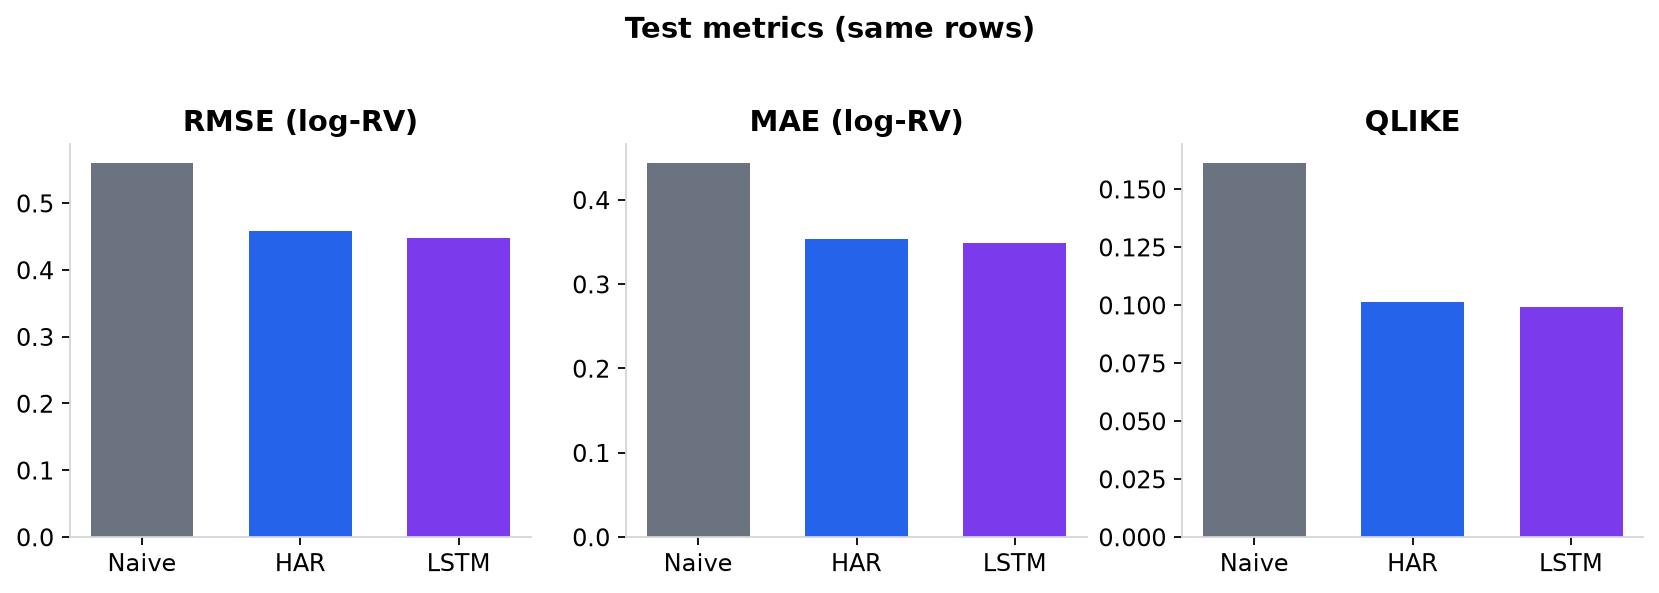
\includegraphics[width=\textwidth]{lstm_test_metrics.png}
\caption{Test RMSE, MAE, MAPE, and QLIKE: Naive, HAR, LSTM.}
\end{figure}

\begin{explain}
The LSTM has the lower test RMSE and MAPE. MAE matches HAR at the reported precision (\(0.354\)). HAR remains lower on QLIKE.
\end{explain}

\begin{figure}[H]
\centering
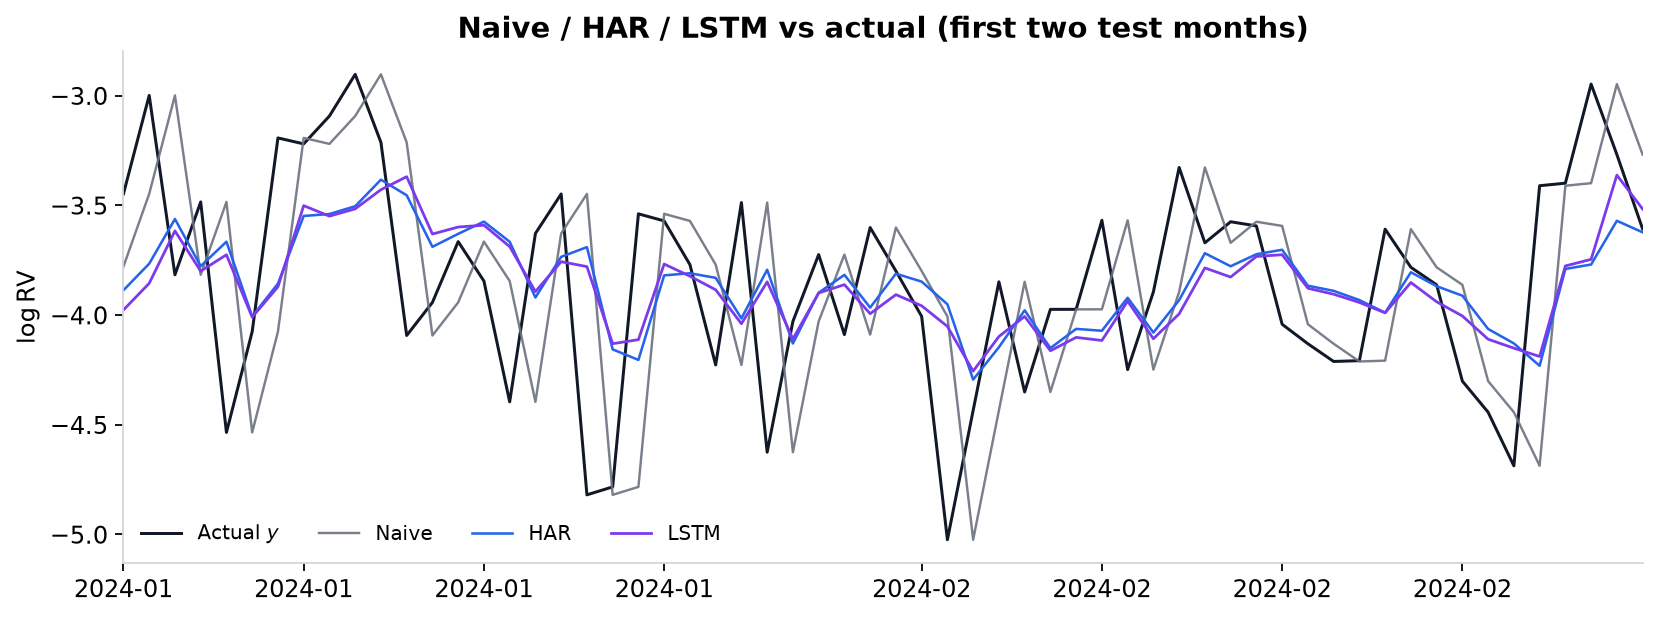
\includegraphics[width=\textwidth]{lstm_test_paths_2mo.png}
\caption{Naive, HAR, and LSTM vs actual (first two test months).}
\end{figure}
\begin{figure}[H]
\centering
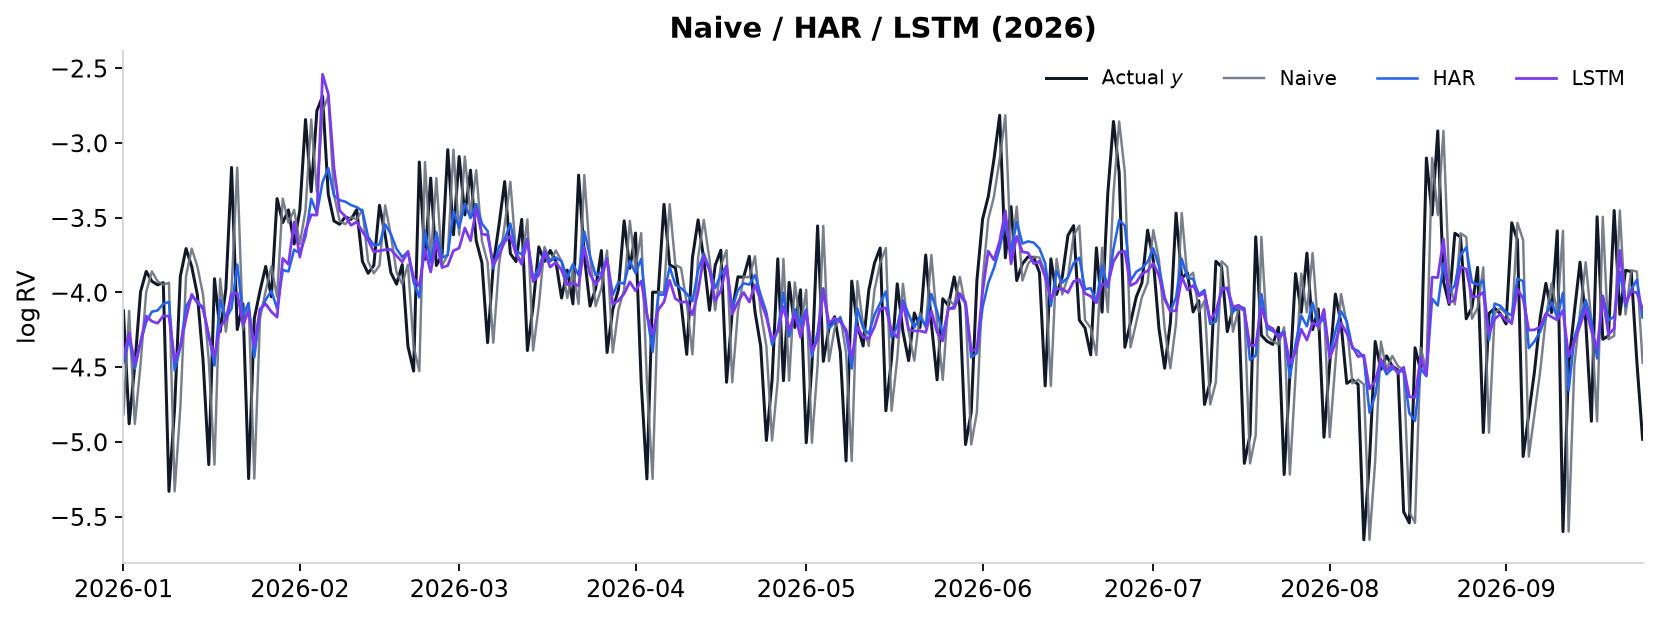
\includegraphics[width=\textwidth]{lstm_test_paths_2026.png}
\caption{Naive, HAR, and LSTM vs actual (calendar 2026).}
\end{figure}

\section{From train to test}
The figure and tables below score the final HAR and LSTM fits on train, validation, and test.
Under Protocol~B those fits use train+val, so the train and validation panels are in-sample.
MAPE in the figure is drawn as a fraction (percent$/100$) so it shares the axis with the other scores.
Bold marks the lower score in each column. No model wins every column on every split.

\begin{figure}[H]
\centering
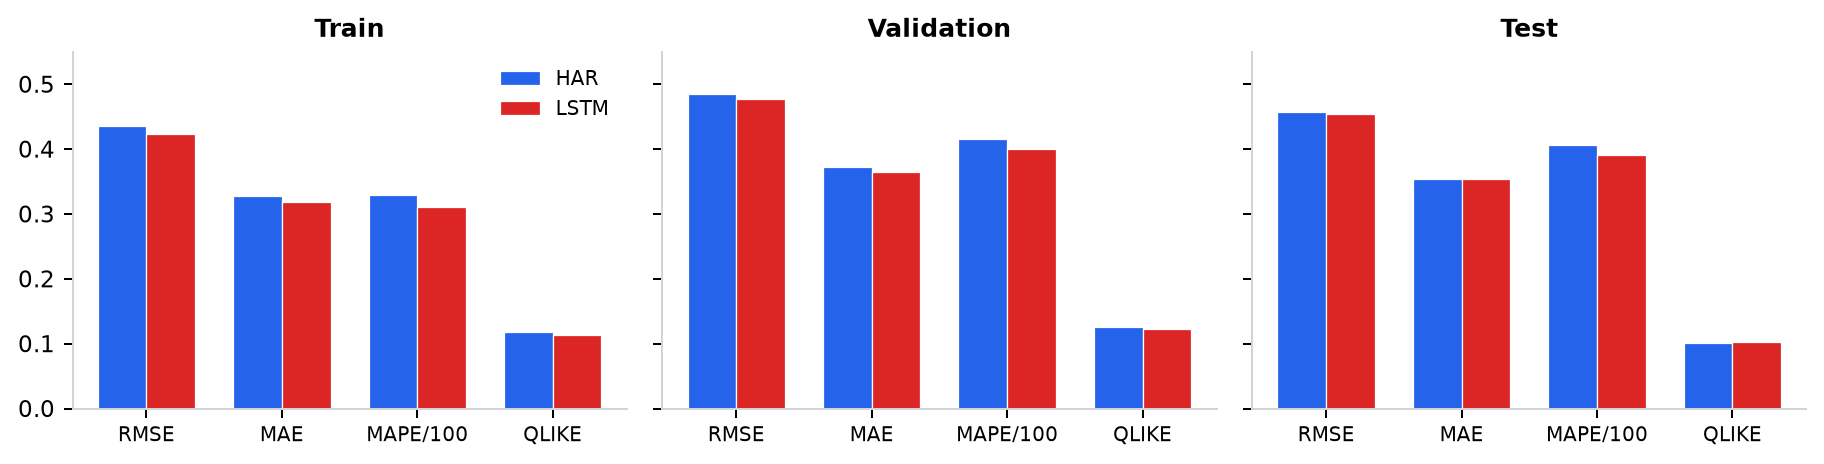
\includegraphics[width=0.92\textwidth]{har_lstm_splits.png}
\caption{HAR vs LSTM on train, validation, and test. Grouped bars are the four scores.
MAPE is shown as a fraction.}
\end{figure}

\begin{table}[H]
\centering
\begin{tabular}{lcccc}
\toprule
Model & RMSE & MAE & MAPE (\%) & QLIKE \\
\midrule
HAR & 0.436 & 0.328 & 33.0 & 0.118 \\
LSTM & \textbf{0.423} & \textbf{0.319} & \textbf{31.0} & \textbf{0.114} \\
\bottomrule
\end{tabular}
\caption{Train. LSTM \(n=1481\) (lookback \(L=60\)); HAR uses all 1540 train rows.}
\end{table}

\begin{table}[H]
\centering
\begin{tabular}{lcccc}
\toprule
Model & RMSE & MAE & MAPE (\%) & QLIKE \\
\midrule
HAR & 0.485 & 0.372 & 41.6 & 0.125 \\
LSTM & \textbf{0.478} & \textbf{0.365} & \textbf{40.0} & \textbf{0.122} \\
\bottomrule
\end{tabular}
\caption{Validation (in-sample under the final train+val fit).}
\end{table}

\begin{table}[H]
\centering
\begin{tabular}{lcccc}
\toprule
Model & RMSE & MAE & MAPE (\%) & QLIKE \\
\midrule
HAR & 0.458 & \textbf{0.354} & 40.7 & \textbf{0.101} \\
LSTM & \textbf{0.454} & 0.354 & \textbf{39.2} & 0.103 \\
\bottomrule
\end{tabular}
\caption{Test (\(n=999\)). On MAE, HAR is \(0.3537\) and the LSTM is \(0.3541\).
Neither model is best on every score.}
\end{table}
\begin{explain}
Early stopping, dropout, a chronological validation grid, and a single test evaluation are already in place.
On train and validation the LSTM leads on every score, but those panels are in-sample after the train+val refit.
On test the picture splits: LSTM on RMSE and MAPE, HAR on MAE and QLIKE.
The network therefore looks clearly stronger in-sample than the clean test edge justifies.
\end{explain}

\section{Is the LSTM win significant?}
Point estimates alone can overstate a small gap. On the test window we run pairwise Diebold--Mariano tests
(Newey--West HAC standard errors, lag \(\lfloor n^{1/3}\rfloor\)) for LSTM versus HAR on the four losses
linked to RMSE, MAE, MAPE, and QLIKE. Details and figures are in \texttt{reports/significance\_report.pdf}.

\begin{table}[H]
\centering
\begin{tabular}{lrrl}
\toprule
Loss & DM & \(p\) & Better \\
\midrule
Squared log-error (RMSE) & $-1.53$ & $0.127$ & n.s. \\
Absolute log-error (MAE) & $+0.19$ & $0.847$ & n.s. \\
Abs.\ \% RV error (MAPE) & $-5.07$ & $<10^{-6}$ & LSTM \\
QLIKE & $+1.57$ & $0.117$ & n.s. \\
\bottomrule
\end{tabular}
\caption{Diebold--Mariano tests, LSTM vs HAR on the test window.
``n.s.'' means not significant at 5\%. Negative DM favors the LSTM.}
\end{table}
\begin{figure}[H]
\centering
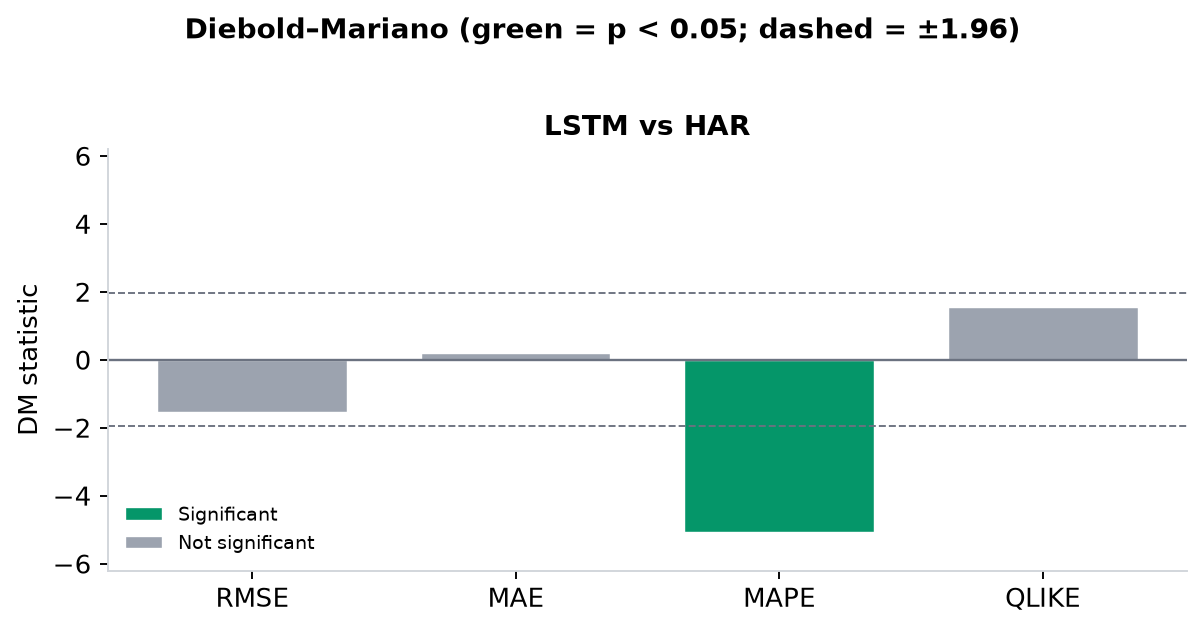
\includegraphics[width=0.82\textwidth]{dm_lstm_vs_har.png}
\caption{DM statistics, LSTM vs HAR. Negative bars favor the LSTM.
Green means significant at 5\%; dashed lines are \(\pm 1.96\).}
\end{figure}
\begin{explain}
The only significant LSTM edge is MAPE. RMSE and QLIKE are not significant; MAE is essentially a tie.
MAPE divides by realized volatility, so calm days get large weight and a small absolute miss becomes a large percentage error.
That MAPE win is real, but it is a weak reason to prefer the standalone LSTM when the main volatility scores
(RMSE, QLIKE) do not show a significant lead.
\end{explain}

\subsection{Why a hybrid}
Two facts motivate a constrained alternative.
First, the standalone LSTM has no significant test win on RMSE or QLIKE; its only significant edge is MAPE, which overweight quiet days.
Second, it leads on every in-sample score while the test edge is thin, which is the pattern of in-sample optimism for a high-capacity model.
Most of the predictable signal in next-day \(\log\mathrm{RV}\) is already the linear day/week/month structure that HAR fits with four coefficients.
A cleaner split of labor is: freeze HAR as that linear component, then train an LSTM only on the residual
\(e_t=y_t-\widehat y_t^{\mathrm{HAR}}\).
The network then spends capacity on what HAR does not explain, instead of re-estimating multi-horizon persistence from scratch.

\section{HAR + LSTM hybrid}
Script: \texttt{models/run\_hybrid.py}.

\subsection{Construction}
\begin{enumerate}
  \item Fit HAR by OLS and freeze the coefficients.
  \item Form the residual \(e_t=y_t-\widehat y_t^{\mathrm{HAR}}\).
  \item Train an LSTM on \(e_t\), with the same channels as the standalone network.
    The linear head is initialized at zero, so the hybrid starts as pure HAR.
  \item Forecast
    \[
    \widehat y_t
    =
    \widehat y_t^{\mathrm{HAR}}
    +
    w\,\widehat e_t^{\mathrm{LSTM}}.
    \]
\end{enumerate}
HAR and the LSTM are not trained jointly. The blend weight \(w\) and the network hyperparameters are chosen on validation; the selected setup is refit on train+val and scored on test once.

\subsection{Selected model}
Same 16-config grid as the standalone LSTM, plus \(w\in\{0.2,0.4,0.6,0.8,1.0\}\) chosen by validation blend RMSE.

\begin{table}[H]
\centering
\begin{tabular}{lr}
\toprule
Setting & Value \\
\midrule
\(L\) (lookback) & 60 \\
Hidden size & 64 \\
Depth & 2 \\
Dropout & 0.1 \\
Learning rate & \(3\cdot 10^{-4}\) (Adam) \\
Blend weight \(w\) & 0.8 \\
Best val epoch & 43 \\
Val blend RMSE & 0.479 \\
\bottomrule
\end{tabular}
\caption{Winning hybrid settings from the validation grid.}
\end{table}

\subsection{Test results}
\begin{table}[H]
\centering
\begin{tabular}{lrrrr}
\toprule
Model & RMSE & MAE & MAPE (\%) & QLIKE \\
\midrule
HAR & 0.458 & 0.354 & 40.7 & 0.101 \\
LSTM & 0.454 & 0.354 & 39.2 & 0.103 \\
Hybrid & \textbf{0.436} & \textbf{0.342} & \textbf{38.3} & \textbf{0.094} \\
\bottomrule
\end{tabular}
\caption{Test metrics. RMSE and MAE on \(\log\mathrm{RV}\); MAPE and QLIKE on RV.}
\end{table}
\begin{figure}[H]
\centering
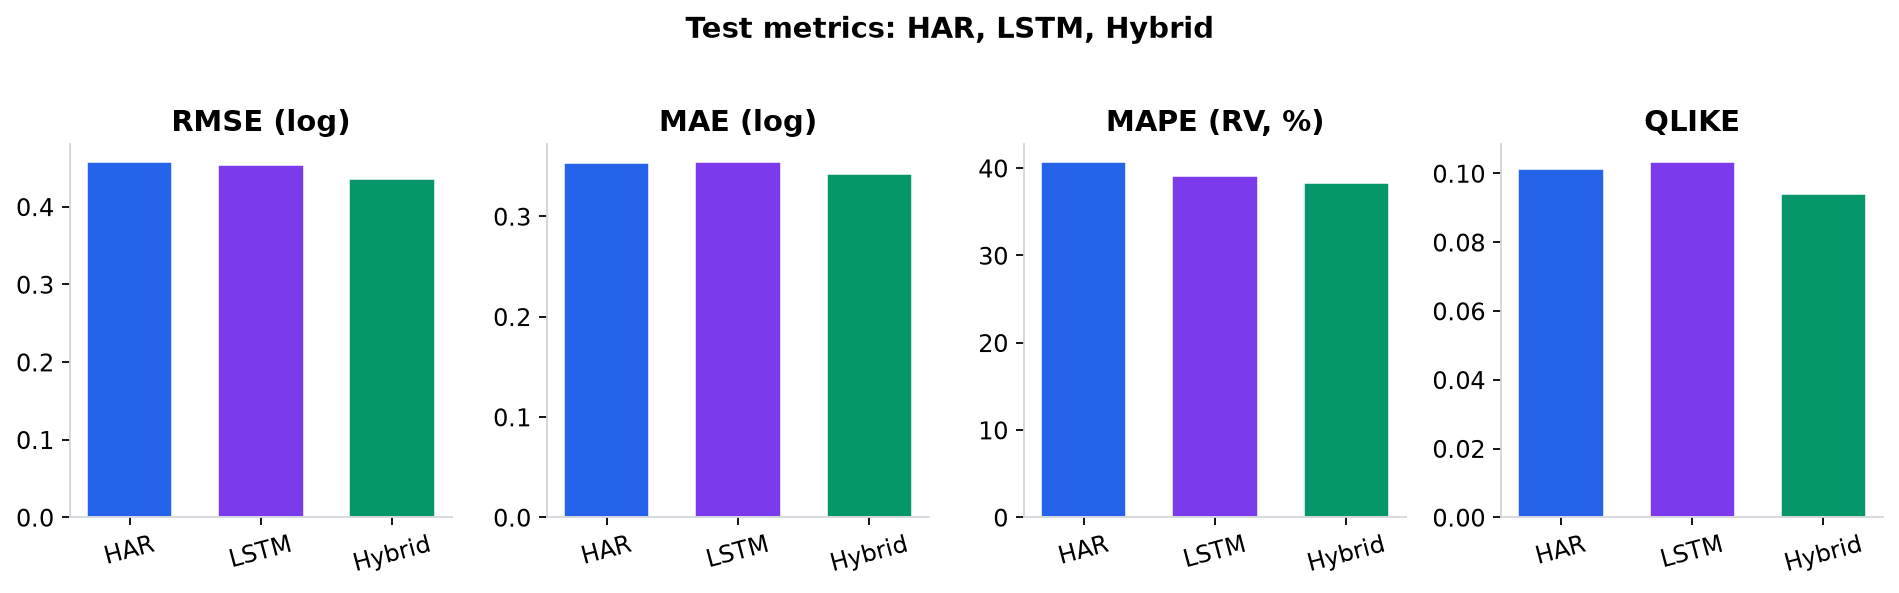
\includegraphics[width=\textwidth]{hybrid_test_metrics.png}
\caption{Test RMSE, MAE, MAPE, and QLIKE: HAR, LSTM, Hybrid.}
\end{figure}
\begin{figure}[H]
\centering
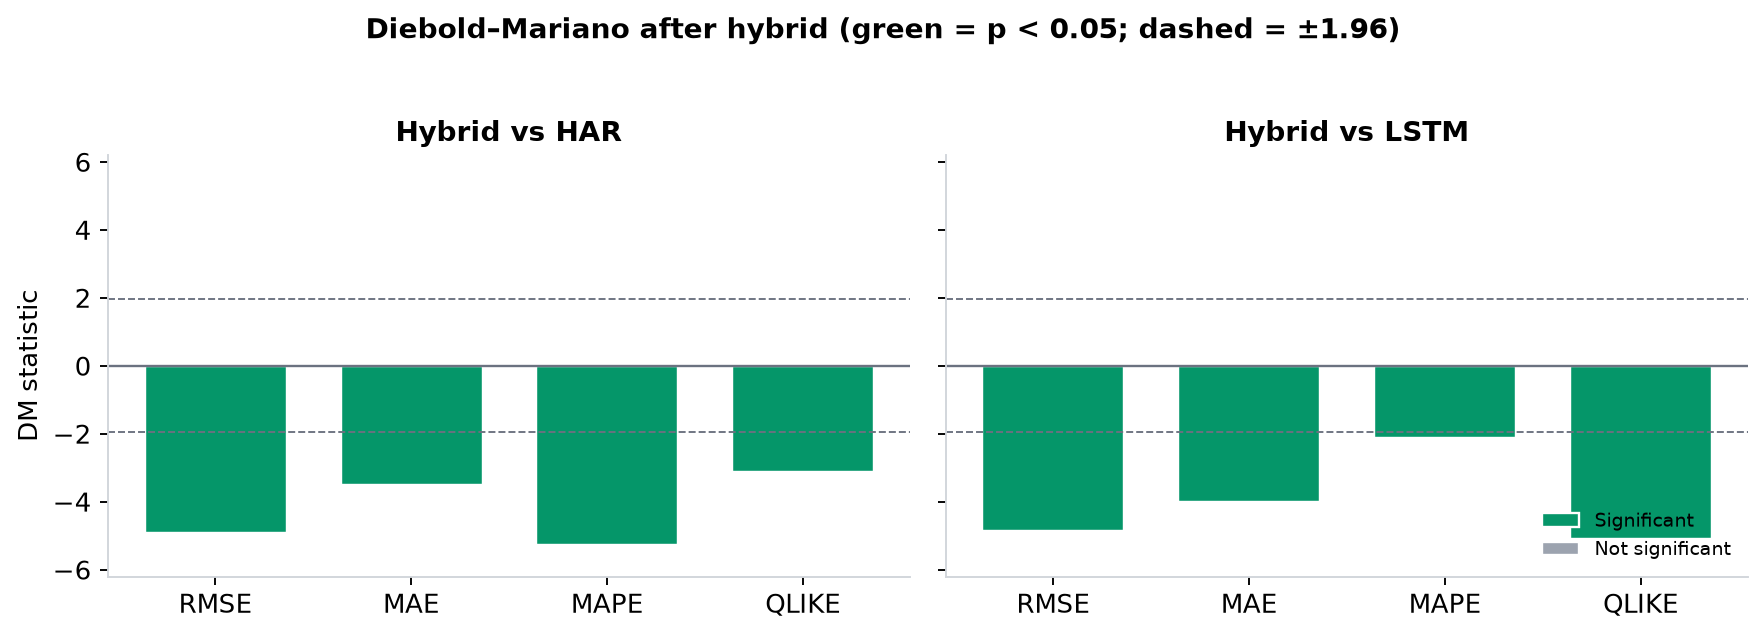
\includegraphics[width=\textwidth]{dm_hybrid_vs_both.png}
\caption{DM statistics after the hybrid: Hybrid vs HAR and Hybrid vs LSTM.
Negative bars favor the hybrid. Green means significant at 5\%.}
\end{figure}
\begin{explain}
The hybrid is lowest on every test score, and the gains are significant against both HAR and the standalone LSTM on all four losses.
Locking the linear multi-horizon fit and training only on the residual is more sample-efficient here than asking the network to do both jobs at once.
\end{explain}
\begin{figure}[H]
\centering
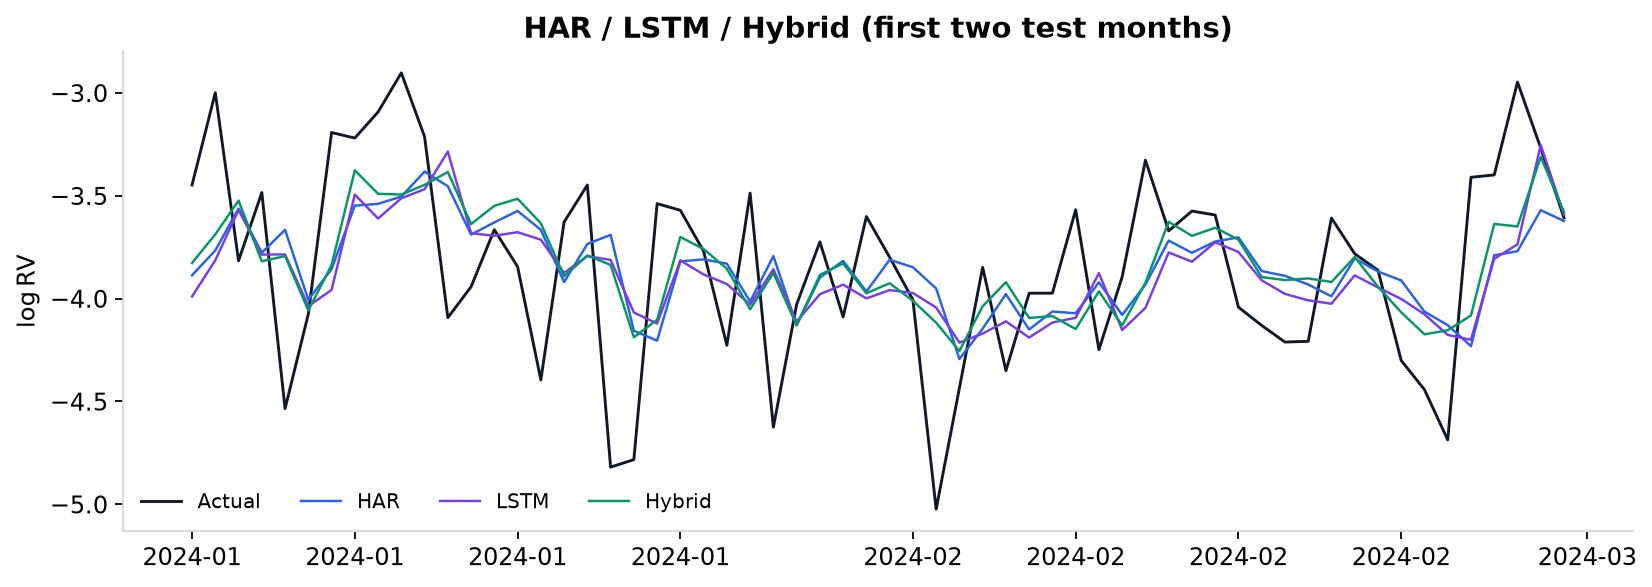
\includegraphics[width=\textwidth]{hybrid_test_paths_2mo.png}
\caption{HAR, LSTM, and Hybrid vs actual (first two test months).}
\end{figure}
\begin{figure}[H]
\centering
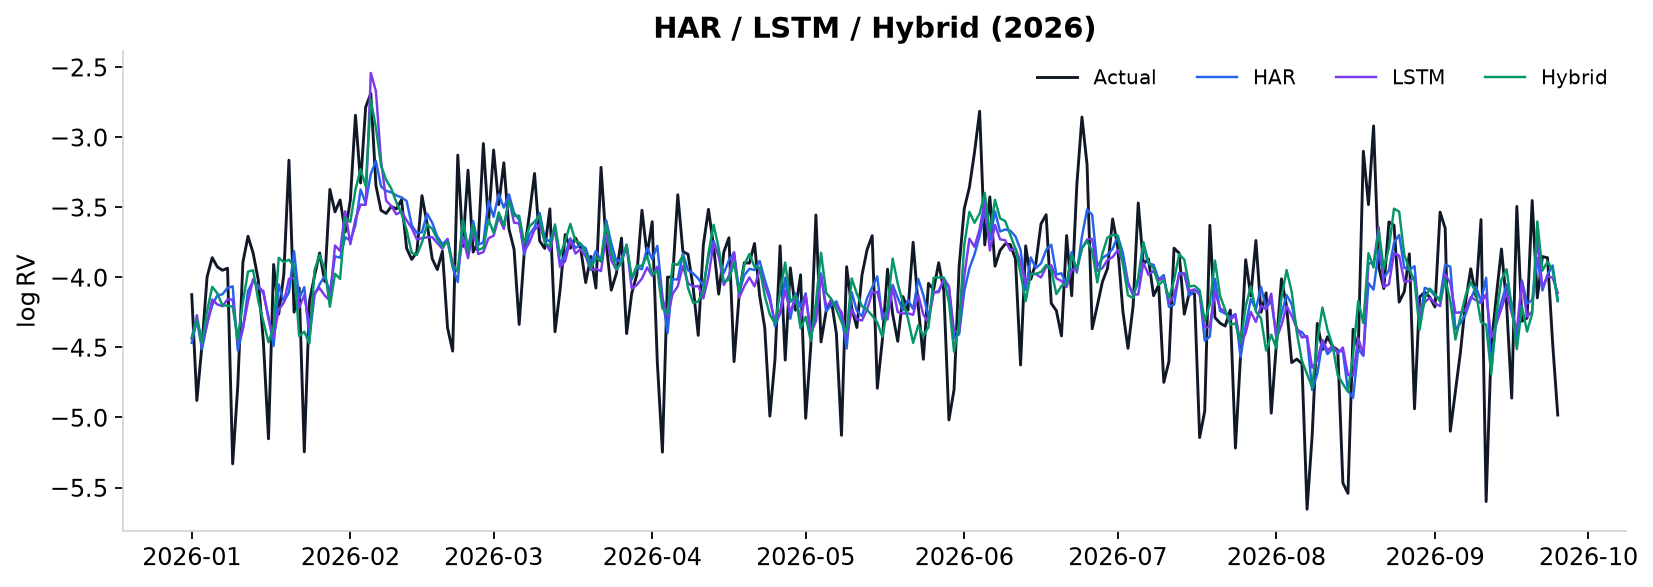
\includegraphics[width=\textwidth]{hybrid_test_paths_2026.png}
\caption{HAR, LSTM, and Hybrid vs actual (calendar 2026).}
\end{figure}

\section{Comparison}
The RV race on one test window and one metric set: Naive, ARIMA, HAR, the standalone LSTM, and the hybrid.
GARCH was scored earlier against Naive and dropped from this board because its forecast object is conditional return volatility, not intraday realized volatility.
Diebold--Mariano tests for HAR, LSTM, and the hybrid are summarized above and in \texttt{reports/significance\_report.pdf}.

\begin{table}[H]
\centering
\begin{tabular}{lcccc}
\toprule
Model & RMSE (log) & MAE (log) & MAPE (\%) & QLIKE \\
\midrule
Naive & 0.560 & 0.444 & 51.1 & 0.161 \\
ARIMA\((3,0,3)\) & 0.518 & 0.407 & 47.4 & 0.132 \\
HAR & 0.458 & 0.354 & 40.7 & 0.101 \\
LSTM & 0.454 & 0.354 & 39.2 & 0.103 \\
Hybrid & \textbf{0.436} & \textbf{0.342} & \textbf{38.3} & \textbf{0.094} \\
\bottomrule
\end{tabular}
\caption{Test window, 1 January 2024 through 25 September 2026, \(n=999\). Bold marks the lowest score in that column.}
\end{table}
\begin{explain}
HAR is the strongest classical RV model. ARIMA improves on Naive and trails HAR. The standalone LSTM is slightly ahead of HAR on RMSE and MAPE, level on MAE, and slightly behind on QLIKE. The hybrid, which freezes HAR and corrects the residual, leads on every score.
\end{explain}

\section{Conclusion}
One-day-ahead \(\log\mathrm{RV}\) is persistent, and most of that persistence is already in the day, week, and month averages. HAR, a four-parameter regression on those averages, is the relevant classical baseline. A standalone LSTM improves point RMSE and MAPE slightly, but Diebold--Mariano finds only the MAPE gap significant; RMSE and QLIKE are not, and the in-sample panels overstate the test edge. Freezing HAR and training an LSTM only on the residual closes more of the gap (test RMSE \(0.436\), QLIKE \(0.094\)) and is significant against both HAR and the standalone LSTM. ARIMA sits between Naive and HAR. GARCH was fit as a return-volatility reference and is not part of the final RV comparison.

\clearpage
\begin{thebibliography}{9}
\bibitem{corsi2009}
F.~Corsi,
``A simple approximate long-memory model of realized volatility,''
\textit{Journal of Financial Econometrics}, vol.~7, no.~2, pp.~174--196, 2009.
\url{https://doi.org/10.1093/jjfinec/nbp001}

\bibitem{goodfellow2016}
I.~Goodfellow, Y.~Bengio, and A.~Courville,
\textit{Deep Learning}.
MIT Press, 2016,
ch.~10.
\url{https://www.deeplearningbook.org/contents/rnn.html}

\bibitem{olah2015}
C.~Olah,
\textit{Understanding LSTM Networks},
\url{http://colah.github.io/posts/2015-08-Understanding-LSTMs/},
2015.
\end{thebibliography}

\end{document}
